\documentclass[a4paper]{article}
\usepackage[top=60pt,bottom=80pt,left=60pt,right=60pt]{geometry}
\usepackage[utf8]{inputenc}
\usepackage[style=phys,url=false,doi=false,isbn=false,eprint=false]{biblatex}
\usepackage{amsmath}
\usepackage{graphicx}
\usepackage{hyperref}
\usepackage{cleveref}
\usepackage{physics}
\usepackage{siunitx}
\usepackage{lipsum}
\usepackage{xurl}

\addbibresource{bibliographies/bib1.bib}
\addbibresource{bibliographies/bib2.bib}
\addbibresource{bibliographies/bib3.bib}
\addbibresource{bibliographies/bib4.bib}
\addbibresource{bibliographies/bib5.bib}
\addbibresource{bibliographies/bib6.bib}
\addbibresource{bibliographies/bibLOQC.bib}
\addbibresource{bibliographies/Introduction.bib}

% Macros for the 0 and 1 kets, might be a useful shorthand, if you want to use it just do \kz or \ko anywhere
\newcommand{\kz}{$\ket{0}$ }
\newcommand{\ko}{$\ket{1}$ }

\begin{document}
\begin{center}
    \Huge \textbf{Building a quantum computer}
\end{center}
\vspace{-1em}

\begin{center}
    \emph{\large All of us}
\end{center}
\vspace{0.5em}
Lengths:\\ \\
Intro + background + Quantum Theory: 10-12 pages\\
Trapped Ions: 15 Pages\\
Photonic Quantum Computers: 10 pages\\
Conclusion: 1-2 Pages\\

\section{Introduction}
A quantum computer uses quantum mechanical phenomena to perform calculations which any classical computer, including supercomputers, would be unable to compute within a lifetime. \cite{noauthor_what_nodate}
This report will explain the physical process and technologies behind building such a machine. Initially, we provide the motivation for wanting to build a quantum computer, which will be followed by an overview of the progress made in both industry and academic research. In order to understand the complex methods used to construct a quantum computer, the report provides explanations of the basic fundamentals of classical computing and the key quantum mechanical concepts, such as entanglement and superposition. Then, we explore a current method for implementing quantum computers - trapped ions, before looking into the next possible breakthrough in the field with linear optical quantum computers.

\subsection{Why build a quantum computer?}\label{sec:why}
In order to understand the power of quantum computers, it is helpful to look to cryptography for an example. Most of computer security in the late 20th and early 21st century has been underpinned by RSA encryption. In the simplest terms, RSA encrypted data has some number, $P$, associated with it, which is a semiprime - it is the product of two prime factors. If you can determine these two factors then you can decrypt the data. If you know one of the factors then it is very easy to find the other, simply by dividing $P$ by the known factor. However, even with some holistic assumption and simplification there is no mathematical formula to compute both factors without any prior knowledge. Therefore, it becomes a case of trial and error which is trivial for a small number such as 15, as you quickly find 5 and 3. However, for a semiprime such as 403135, there are a many more possible factors to trial. In fact, modern RSA encryption uses semiprimes comprising over 1000 digits.

A typical classical computer with $n$ bits can represent $2^n$ different values, so in theory could trial $2^n$ factors. It would process each trial value sequentially. If we take the computation time for trialling one value to be constant, then the entire processing time scales as $2^n$. Therefore, for RSA encryption using significantly large semiprimes, the vast number of factors necessary to trial makes the computation time so long that the the encrypted data is effectively secure. It would take a classical computer 300 trillion years to trial all possible factors necessary to break RSA encryption using a semiprime of approximately 600 digits, as you would need a classical computer with 112 bits \cite{mahto2016security}\cite{quintessencelabs_2022}.
made 
This is where a quantum computer comes in. A quantum computer with $n$ qubits (quantum bits) can also represent $2^n$ different values, however, it can do so simultaneously. This is possible because of quantum mechanical phenomena such as superposition. If a quantum computer can try all possible factors at once, the processing time is now a constant. Therefore, a 112 qubit quantum computer could, in constant time, break the 600 bit RSA encryption that would take a classical computer 300 trillion years to solve.

This incredible processing power makes quantum computers ideal at solving many other combinatorics based problems, where finding the solution involves trying a vast number of possibilities. Two particularly interesting applications are in financial and medical simulation. Monte Carlo simulation calculates the likely outcome of a certain event by running enough simulations that it covers a suitable range of possibilities; these repeated simulations are equivalent to trialling different factors for RSA encryption. Goldman Sachs has invested heavily in this technology, and executed a quantum version of its Monte Carlo simulation on a trapped ion computer - they believe it will allow traders to obtain up-to-date risk predictions 10 times faster within the next five years \cite{Giurgica_Tiron_2022}. Quantum computers also have the potential to rapidly advance drug development by allowing researchers to test many different combinations of atoms and molecules simultaneously \cite{bova2021commercial}.

If you want a computer to watch YouTube or write a word processing document, then a quantum computer probably isn't necessary for you. However, if you want to accelerate humanity's innovation in medicine, physics, finance, cybersecurity and more, hopefully it's now clear why you should build a quantum computer.

\subsection{Current Methods of Quantum Computing}
There are multiple method to building a quantum computer and no single method is the leading approach.
Superconducting qubits (qubits are the quantum realisation of classical bits) is the method currently being researched by IBM, Google and a select few others and it was the first method to claim quantum supremacy. \cite{gibney_hello_2019}
Quantum supremacy is a term used to describe when a quantum computer is able to complete a calculation that a classical computer could not achieve in a reasonable amount of time. 

Google was first to claim it in 2019 with their 53 bit `Sycamore' quantum computer which reportedly solved a problem in under 5 hours which would take a classical computer over $10\text{ }000$ years.\cite{gibney_hello_2019} 
However these claims were disputed by IBM - another large company heavily invested in the quantum computing race.
The largest quantum computer to date is the IBM osprey with 433 qubits announced in November 2022.\cite{irving_ibm_2022}

This report will instead focus on trapped ion systems. 
One of the largest contenders in this area is IonQ with a 23 qubit computer. 
 Although trapped ions systems have not yet reached the number of qubits as seen from superconducting systems there are many advantages such as: 
\begin{itemize}
    \item The cost of ion trap systems is relatively low - therefore research can be carried out by academics and be peer-reviewed. As opposed to superconducting systems which require vast investments, leading to only a select few companies willing to research this approach. Therefore significantly more detailed research is available on ion trapped systems.  
    \item Many small (tens of qubits) quantum computers have been built using trapped ion systems. It fulfils all the requirements for a quantum computer however it is a difficult to scale to hundreds of qubits. See section \ref{sec:Trapped}
    \item The company IonQ produces commercially available quantum computer using trapped ion systems which can be accessed from public clouds such as Microsoft Azure. \cite{sonialopezbravo_ionq_nodate} Goldman Sachs have been using this service to test quantum algorithms relevant to the financial services industry. \cite{noauthor_goldman_2021}
\end{itemize}




The next section in this report will provide some background information and explain some key fundamential ideas in classical computing and quatum information. 
The following section will then venture into trapped ion systems where quantum computers have been built using this method.
It will cover how physical qubits are created and manipulated using gates for calculations to be carried out and finally how the qubit states can be readout. 


Lastly the report will discus optical qubits due to their likely scalability for the future. 
Quantum computers are likely to require up to millions of qubits for most quantum algorithms - as compared to the current record of 433 qubtis from IBM. \cite{bergou_quantum_2021} 
Optical qubits currently have some large hurdles to overcome - as will be discussed in section \ref{sec:Photonic}. 
However once these are overcome it is likely to be an attractive attender for future quantum computing and information transfer.
In particular, photons can maintain entanglement over long distances and time periods allowing secure transition of quantum information - this has been demonstrated for over 1200km. \cite{yin_satellite-based_2017}
\section{Background}

This section will cover some of the fundamental concepts both in quantum mechanics and classical computing which are required for understanding this paper. 
Finally the DiVincenzo criteria will be introduced which is five objectives that should be met by any system in order to be an effective large scale quantum computer. 

\subsection{Fundamentals of Classical Computing}
Quantum computers are an extension of the founding principles of classical computation, which take advantage of quantum mechanical phenomena. Therefore, in order to understand how to build a quantum computer, it is beneficial to have a strong understanding of a classical computer's basic components. In order to build a functioning quantum computer, every fundamental feature described in the sections below must have an analogous, albeit quantum, implementation.
\subsubsection{What is a bit? Or a nibble, or even a byte...}
In computing the smallest unit of information is known as a bit, and can take a value of 1 or 0. This is because computers work in a binary number system as opposed to the decimal system one learns as a child, where a single digit can take values from 0 to 9. The major motivation behind this was for ease of implementation; it is much easier to create a switch that can be on or off than one that has 10 different positions. 

Individual bits don't allow us to represent much, however, we can chain them together to represent larger and larger numbers. We call a group of four bits a nibble, and more commonly known is a group of eight - a byte. Figure \ref{fig:BINARY} illustrates how six bits are combined to make the number 45, where digits further to the left show contributions from higher powers of 2.
\begin{figure}[H]
    \centering
    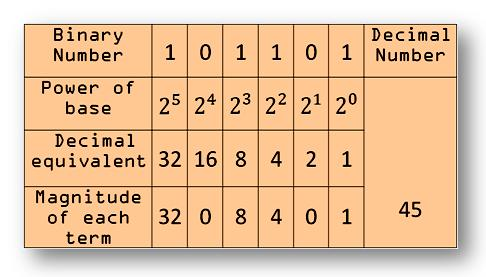
\includegraphics[width=0.6\textwidth]{images/binary.jpg}
    \caption{A table illustrating how to convert the binary number 101101 into its decimal equivalent, 45 \cite{binary}}\label{fig:BINARY}
\end{figure}

Clearly bits are a good way of representing numbers, however, they can also be mapped to other useful properties. For example, we can represent a text file by assigning a bit pattern to each letter. Or, we could apply our computer to DNA simulation using 2 bits to represent each of the four chemical bases. 

\subsubsection{How is a bit physically stored?}
In order to represent a bit, it must be possible to distinguish between two distinct states; like a light switch which can be off or on. Classical computers are formed of many complex, intricate electrical components. Therefore, it makes sense to represent bits as an electrical voltage. In a simple explanation, we can consider a bit with value 0 to be when there is no voltage (the ground state) and a bit with value 1 to be when the voltage is equal to the supply voltage. In practice, there is tolerance of approximately 30\% about these states \cite{voltage}.

It is important to point out, that the essence of building a quantum computer lies in the method of physically representing the quantum analogy to bits (qubits). 

\subsubsection{Gates - Manipulating bits}
Clearly bits can be used to represent different values or states, however, it is their processing and manipulation which allows for computation. Gates are components which take one or more bits as input, and output a single bit with a state dependent on the input values. Figure \ref{fig:ANDGATE} shows the diagrammatic symbol for an AND gate along with all of its possible outputs. The AND gate will output 1 only if both of its inputs are also 1 (otherwise it outputs 0).
\begin{figure}[H]
    \centering
    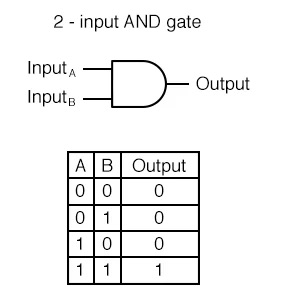
\includegraphics[width=0.4\textwidth]{images/andgate.jpeg}
    \caption{The circuit symbol for an AND gate, along with a truth table of all possible outputs for two inputs, A and B. \cite{andgate}}\label{fig:ANDGATE}
\end{figure}

There are many other gates, such as the NOT which takes a single bit as input and outputs a bit with the opposite state. The important point to highlight is that gates provide building blocks for computation.

\subsubsection{Computation - Many gates}
Computer algorithms can be boiled down to passing bits through a circuit of different gates. 
\begin{figure}[H]
    \centering
    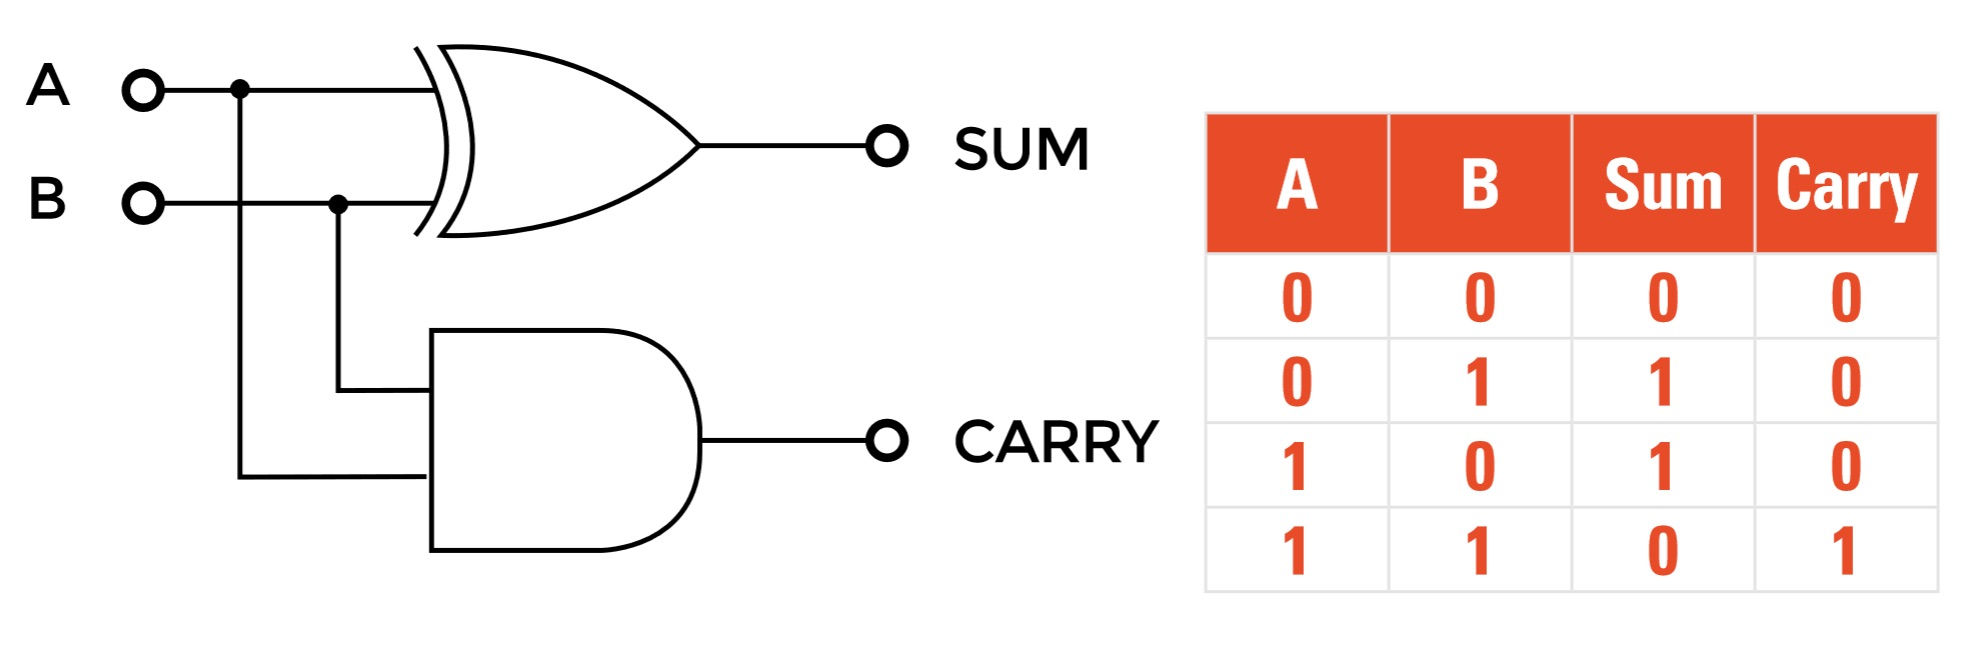
\includegraphics[width=0.7\textwidth]{images/adder.jpeg}
    \caption{A logic diagram of a binary half adder, including truth table output for all possible input combinations. \cite{adder}}\label{fig:ADDER}
\end{figure}

 The ability to implement gates and process bits using them, is a fundamental pillar of computation whether that be classical or quantum. The report will know introduce concepts from quantum physics which are core to understanding how to build a quantum computer. With this knowledge, it will then be possible to draw analogies between classical and quantum computing implementations.

\subsection{Relevant Quantum Physics}

Quantum computing's advantages are a direct result of the quantum mechanical properties such as superposition and entanglement that distinguish it from classical computers. 
These two properties will be discussed, then decoherence times of quantum states will be introduced as a means of demonstrating the difficulty with scailability in quantum computing. 


\subsubsection{Superposition}\label{sec:superposition}
Superposition is a quantum mechanical phenomenon where an object may exist in multiple states at once. 
For example an electron may be said to be in two places at once - or more accurately its probability function covers multiple areas in space. \cite{noauthor_whatCal_nodate}

Superposition can be observed in the polarisation of light. 
Light can be horizontally, vertically and circularly polarized and much of the light around us is a superposition of the three.
However when light interacts with surfaces their properties can change such as light reflecting off a pond being horizontally polarized. 
Using a linear polariser one can control the direction of polarisation of the light passing through it.
Constructing two polarisers at right angles (horizontal and vertical respectively) one would expect only horizontal polarised light to emitted from the first and then no light to be emitted from the second polariser. 
This is what is experimentally observed - however if a third polariser is placed between the horizontal and vertical polarisers orientated at 45$^\circ$ (as in figure \ref{fig:polarisers}) from both then light will now be transmitted through the final horizontal polariser (at 50$\%$ intensity). \cite{noauthor_whatCal_nodate}

\begin{figure}[H]
  \centering
  \begin{subfigure}[t]{0.4\textwidth}
    \centering
    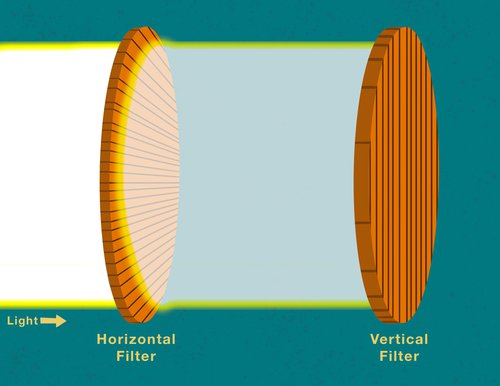
\includegraphics[width=\textwidth]{images/2 polariser.jpg}
    \caption{Unpolarised light passing through a horizontal and then failing to pass through a vertical polarising filter.}\label{fig:2 polarise}
  \end{subfigure}
  \begin{subfigure}[t]{0.4\textwidth}
    \centering
    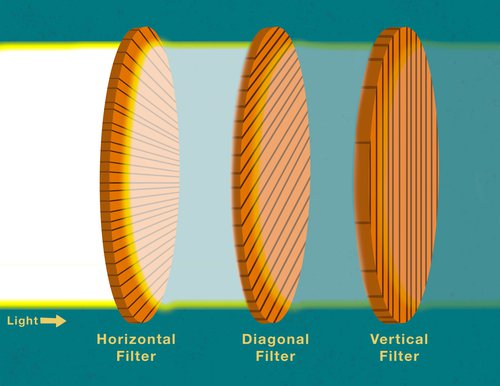
\includegraphics[width=\textwidth]{images/3 polariser.jpg}
    \caption{Unpolarised light passing through three successive polarising filters. A horizontal and vertical filter and a linear polariser orientated 45$^\circ$ between both. }\label{fig:3 polarise}
  \end{subfigure}
  \caption{Unpolarised light passing through linear polarising filters in two set ups. \cite{noauthor_whatCal_nodate}}
  \label{fig:polarisers}
\end{figure}
This also emphasises this highly probabilistic behavior of QM where after exiting the second polariser the light is in a superposition of the states which allow diagonal polarisation - some of which is vertical and therefore can pass through the final filter.
It is this superposition of states which allows a single qubit to trial multiple values at once. \cite{sonialopezbravo_understanding_nodate}


\subsubsection{Entanglement}
Entanglement is a uniquely quantum mechanical phenomenon where the measurement of one particle's state will effect the state of another particle.
I.e. for interacting states A and B their combined wavefunction cannot be expressed as the product of the individual wavefunctions of A and B if states A and B are entangled. \cite{bransden_quantum_2000}

For example the LHS of equation \ref{eqn:superqubit} is not an entangled system (simply a superposition of states) as it can be expressed as the tensor product of both wavefunctions $|phi\rangle$ and $|psi\rangle$.

\begin{equation}\label{eqn:superqubit}
    |0\rangle_\phi|0\rangle_\psi + |0\rangle_\phi|1\rangle_\psi + |1\rangle_\phi|0\rangle_\psi +
    |1\rangle_\phi|1\rangle_\psi = |\phi\rangle \otimes |\psi\rangle
\end{equation}

However the system in equation \ref{eqn:entqubit} is entangled as the total system cannot be expressed as a product of the two single systems. 
\begin{equation}\label{eqn:entqubit}
    |0\rangle_\phi|0\rangle_\psi + 
    |1\rangle_\phi|1\rangle_\psi
\end{equation}



Although progress has been made in studying quantum entanglement, there is no complete theory to explain it. 
It does play an integral role in quantum computing however and deeper investigation of it and how to manipulate this property is likely to lead to further applications. \cite{nielsen_quantum_2010}



\subsubsection{Decoherence of States}
Decoherence is when a quantum state collapses into a single state i.e. no longer a superposition.
This is a consideration in quantum computing as qubits are fragile and decoherence may occur.
It is especially challenging when trying to scale up to large multi-qubit operations and maintain control over the system. \cite{zhang_observation_2017}
Quantum systems can have a `lifetime', $T_2$ after which the state `relaxes' into a classical single state. 
Therefore a good physical system for quantum computing must have a long $T_2$ and have operations (gates) which are unlikely to cause decoherence. \cite{nielsen_quantum_2010}



\subsection{Quantum Computing}
\subsubsection{Qubits}
Following the explanation of bits in a classical computer, a qubit is the quantum analogy to a classical bit. Qubits are crucical to perfoming calculations on a quantum computer but have fundamental variation on their classical counterpart.
A classical bit can either hold the value of 0 or 1 while a qubit is a superposition of both $|0\rangle$ and $|1\rangle$ as seen in equation \ref{eqn:qubit}
\begin{equation}\label{eqn:qubit}
    |\psi\rangle = \alpha|0\rangle + \beta|1\rangle
\end{equation}
where $\alpha$ and $\beta$ are complex numbers such that $|\alpha|^2 + |\beta|^2 = 1$.
Operations can be preformed on this superposition state and only once the qubit has been measured the state will collapse to either $|0\rangle$ or $|1\rangle$. \cite{nielsen_quantum_2010}
The matrix representations of the $|0\rangle$ and $|1\rangle$ states can be seen in equation \ref{eqn:qmatrix} and is useful for understanding gate operations.

\begin{equation}\label{eqn:qmatrix}
    |0\rangle = \begin{bmatrix}
1 \\
0 
\end{bmatrix} \text{ and } |1\rangle = \begin{bmatrix}
0 \\
1 
\end{bmatrix}  
\end{equation}

Qubits can also be represented as a vector within a radius 1 bloch sphere and represented by angles $\theta$ and $\phi$ as opposed to the complex numbers $\alpha$ and $\beta$, see equation \ref{eqn:bloch}

\begin{equation}\label{eqn:bloch}
    |\psi \rangle = \cos \frac{\theta}{2}|0\rangle + e^{i \phi}\sin \frac{\theta}{2} |1\rangle
\end{equation}

The visual representation of a Bloch sphere can be seen in figure \ref{fig:bloch}.
This is a particularly helpful way of visualising qubits with regards to gate operations as they can be seen as rotations and reflections within this sphere. \cite{noauthor_representing_nodate}


\begin{figure}[H]
    \centering
    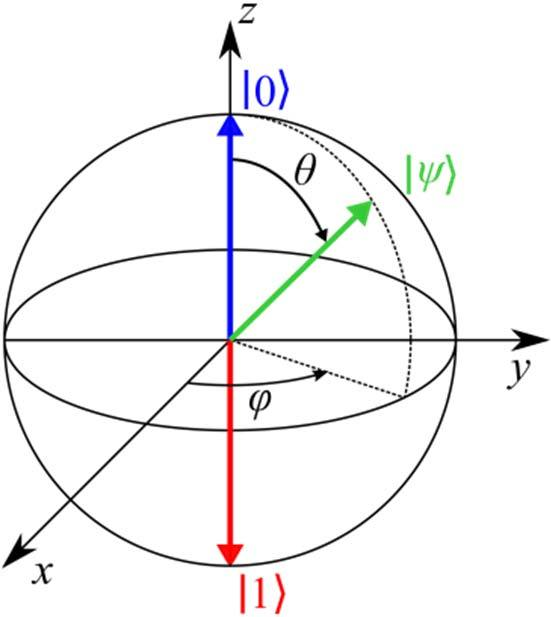
\includegraphics[scale=0.3]{images/Bloch-sphere-representation-of-a-qubit.png}
    \caption{Diagram of a Bloch sphere - 
 representing a qubit as a vector. x-axis is $\frac{|0\rangle + |1\rangle}{\sqrt{2}}$ and y-axis is $\frac{|0\rangle+i|1\rangle}{\sqrt{2}}$.\cite{sebastiano_cryo-cmos_2017}}. \label{fig:bloch}
\end{figure}

As with classical computing, quantum computing requires gates to preform basic manipulation of qubits. 
Calculations are then preformed by using these gates in series.
Quantum gates must be able to modify the probabilities without decoherence or collapse of the wavefunction. 
In the next sections, a selection of common single and two qubit gates are introduced.
The universal set of quantum gates is explained which can be comprised of the gates in section \ref{sec:singlequbit} and \ref{sec:twoqubit}  

\subsubsection{Single Qubit Gates}\label{sec:singlequbit}
Single qubit gates are ones which act on only one qubit. 
This section will describe the Hadamard, Phase Gate and the three Rotation gates. 

{\bf Hadamard gate} is represented as a rotation about the y-axis of 90$^\circ$ and x-axis of 180$^\circ$ of figure \ref{fig:bloch}.
The matrix representation of this is in equation \ref{eqn:hadamard}. 

\begin{equation}\label{eqn:hadamard}
    H = \frac{1}{\sqrt{2}} \begin{bmatrix}
1 & 1 \\
1 & -1 
\end{bmatrix}  
\end{equation}
The effect of this gate on a qubit is seen in equation \ref{eqn:qH}.
i.e. it turned the $|0\rangle$ state into a equal superposition of $|0\rangle$ and $|1\rangle$ - the same happened to the $|1\rangle$ state.
\begin{equation}\label{eqn:qH}
    \left( \alpha \begin{bmatrix}
1 \\
0 
\end{bmatrix}  + \beta  \begin{bmatrix}
0 \\
1 
\end{bmatrix}   \right) \cdot \frac{1}{\sqrt{2}} \begin{bmatrix}
1 & 1 \\
1 & -1 
\end{bmatrix} = \alpha \frac{|0\rangle +|1\rangle}{\sqrt{2}} + \beta \frac{|0\rangle - |1\rangle}{\sqrt{2}}
\end{equation}


{\bf Phase gate} is a rotation about the z-axis of figure \ref{fig:bloch} for the $|1\rangle$ state and requires an angle $\phi$. 
The matrix representation of this is in equation \ref{eqn:phase}.
\begin{equation}\label{eqn:phase}
    P =  \begin{bmatrix}
1 & 0 \\
0 & e^{i \phi}
\end{bmatrix}  
\end{equation}
The effect of this gate on a qubit is seen in equation \ref{eqn:qP}.
\begin{equation}\label{eqn:qP}
    \left( \alpha \begin{bmatrix}
1 \\
0 
\end{bmatrix}  + \beta  \begin{bmatrix}
0 \\
1 
\end{bmatrix}   \right) \cdot \begin{bmatrix}
1 & 0 \\
0 & e^{i\phi} 
\end{bmatrix}  = \alpha |0\rangle + \beta e^{i\phi}|1\rangle
\end{equation}

There are {\bf three rotation} gates $R_x(\theta)$, $R_y(\theta)$ and $R_z(\theta)$ for rotations of the Bloch sphere (figure \ref{fig:bloch}) about the x, y and z axes respectively. 
\begin{equation}
    R_x(\theta) = \begin{bmatrix}
\cos (\theta/2) & -i \sin (\theta/2) \\
-i \sin (\theta/2) & \cos (\theta/2) 
\end{bmatrix}  
\end{equation}
\begin{equation}
    R_y(\theta) = \begin{bmatrix}
\cos (\theta/2) & - \sin (\theta/2) \\
\sin (\theta/2) & \cos (\theta/2) 
\end{bmatrix}  
\end{equation}
\begin{equation}
    R_z(\theta) = \begin{bmatrix}
\exp (-i \theta/2) & 0 \\
0 & \exp (i \theta/2) 
\end{bmatrix}  
\end{equation}
Some gates that we can expect to encounter a lot are the Pauli X, Y and Z gates. These gates are special cases of the three rotation gates where $R_{x,y,z}(\pi) = -i\{X,Y,Z\}$. In matrix form these look like:
\begin{equation}
    X = 
    \begin{bmatrix}
        0 & 1\\
        1 & 0\\
    \end{bmatrix}, \\
    Y = 
    \begin{bmatrix}
        0 & -i \\
        i & 0 \\
    \end{bmatrix},\\
    Z = 
    \begin{bmatrix}
        1 & 0 \\
        0 & -1 \\
    \end{bmatrix}
\end{equation}

\subsubsection{Two Qubit Gates}\label{sec:twoqubit}
Similar to classical computing there requires to be gates that act on multiple qubits for calculations to be preformed. 
The quantum two bit gate is known as a controlled NOT or CNOT gate, where one qubit is the `control' qubit and the other is the `target' qubit. \cite{nielsen_quantum_2010}
A two qubit state can be represented by $|\psi\rangle = \alpha |00\rangle + \beta|01\rangle + \gamma|10\rangle + \delta |11\rangle$ with $|ij\rangle=|i\rangle \otimes |j\rangle$ where $i$ is the control and $j$ is the target. 
Note the notion of some two qubit states are represented as $|01\rangle = |2\rangle$ and $|11\rangle$.

The matrix representation of the CNOT gate can be seen in equation \ref{eqn:CNOT}.

\begin{equation}\label{eqn:CNOT}
    \begin{bmatrix}
1 & 0 & 0 & 0 \\
0 & 1 & 0 & 0 \\
0 & 0 & 0 & 1 \\
0 & 0 & 1 & 0 
\end{bmatrix}  
\end{equation}
The effect of the CNOT gate is that if the control qubit is in state $|0\rangle$ then the state of the target qubit is unchanged, however if the state of the control qubit is $|1\rangle$ then the state of the target qubit is flipped. 
For each state the following occurs $|00\rangle \Rightarrow |00\rangle$, $ |01\rangle \Rightarrow |01\rangle$, $ |10\rangle \Rightarrow |11\rangle$ and $|11\rangle \Rightarrow |10\rangle$.


\subsubsection{The Universal Set of Quantum Gates} \label{sec:USoQG}
As in classical computing, quantum algorithms are executed as qubits are passed through and manipulated by a series of consecutive gates. 

The state in equation \ref{eqn:entqubit} (with a factor of $1/\sqrt{2}$) is an interesting illustration of this; it is known as the Bell state, which is 2 qubit entanglement frequently used in quantum computations. The Bell state is formed by applying a Hadamard gate to a qubit, which then acts as a control input for a CNOT gate. The CNOT is applied to this control and another, target, qubit. \cite{mermin_quantum_2007} 
By measuring one of the qubits in the Bell state, one can then reveal the state of the other qubit. If a $|0\rangle$ is measured then the other qubit must be $|0\rangle$ and vice versa. The probability of measuring $|0\rangle$ is 50$\%$ and similarly for measuring $|1\rangle$. 

There are many quantum gates beyond those described so far, including the Toffoli, Controlled-Z and more. However, it can be mathematically proven that a small subset of the quantum gates can be combined to make any of the others. This is known as a universal set. Therefore, a physical quantum computer needs only to implement all of the gates in this set, in order to guarantee that any desired computation is attainable \cite{universalset}.

There is no one universal set of quantum gates, and the choice of which gates to implement is likely dependent on the kinds of calculations the computer will be used for, as well as the practicality given a choice of technology. However, to provide an example, the most commonly used universal set of quantum gates is composed of the CNOT, phase gate and the rotation gates.

\begin{equation}
    Universal\ Set = \{ R_x, R_y, R_z, Ph, CNOT \}
\end{equation}

In fact, it is only necessary to use two of the three rotation gates.

\subsubsection{The DiVincenzo Criteria}\label{sec:DiVincenzo}
In 2000, the components of a quantum computer, which are introduced in the sections above, were formalised into the DiVincenzo criteria. These are a list of seven objectives that must be fulfilled in order to construct a physical quantum computer. This report will not focus on the final two criteria as they are only necessary for quantum communication, rather than computation \cite{bergou_quantum_2021}.

The report will show how possible technologies for implementing a quantum computer are able to satisfy the following five DiVincenzo criteria.
\begin{enumerate}
    \item Scalability with well defined qubits
    \item The ability to initialise the system in a well defined, determinate state
    \item The ability to read out qubit state with high accuracy
    \item A set of universal quantum gates
    \item Long relevant decoherence times
    \newcounter{enumTemp}
    \setcounter{enumTemp}{\theenumi}
\end{enumerate}

The first objective requires qubits to be in a superposition of two clearly defined states. For example, as a superposition of vertical and horizontal polarisation of light. The greater challenge in the first criterion is that of scalability; in order to unlock the power of quantum computing, it is necessary to have many entangled qubits operating on the same problem.

The second objective is to initialise the qubits into a well defined determinate state i.e. initialise the qubit register so all are in the 0 state $\vert 0\rangle \vert 0\rangle$...$\vert 0 \rangle$. \cite{lapierre_divincenzo_2021}

The third objective is to read out qubit state $\vert 0\rangle$ or $\vert 1 \rangle$ with high accuracy. Measurement that have a higher propbability of error can be repeated in order to mitigate this effect.

The fourth objective is to implement a universal set of gates, as explained above. If an implementation includes all gates in a universal set, then such a computer could emulate any sequence of quantum gates, thus executing any desired  quantum algorithm. This is in many ways a positive simplification for building a quantum computer, as it only requires the assembler to create a few important gates. 

The final objective is for long `relevant' decoherence times; this requires the qubit to stay in a superposition for longer than the duration of gate operations before the state collapses. Without this condition, there would not be a long enough time for taking useful measurements.


\section{Trapped Ion Quantum Computing} \label{sec:Trapped}
In this section we provide an introduction to the implementation details of trapped ion quantum computers (**once done possibly elaborate what exactly we covered).
The qubits in a trapped ion system are represented by individual trapped ions, as would have been seen in a quantum mechanics class, electrons bound in atoms can occupy a certain number of possible quantum states, here 2 of these level are chosen and used as the \kz and \ko states.
Though it isn't quite as simple as that, for quantum computing we must have a way of entangling these 2 states.
To achieve that, the qubits are trapped in the same trap (explained later on) and their motion within it is coupled as a quantum system, through which entanglement is achieved.
Finally for qubit manipulation, lasers are used to excite and cool down the electrons and the ions themselves.

\subsection{Ion Trapping and the Paul Trap}
Ion trapping is an extensive field of expertise used for many purposes across physics and other sciences, it is an essential component of many devices and experiments that try to manipulate individual particles, molecules or so on.
For a brief sketch of what this involves, these experiments must be done in vacuum (otherwise there would be too many other atoms around) and rely on complex electric and magnetic fields to manipulate the motion of charged atoms.
For quantum computing we are interested in trapping individual ions in a stable way, and while we want to trap multiple of them (currently about 5-100 has been achieved !43) it is important that we can tell them apart (as opposed to trapping them in bunches as is often done).

There are currently 2 dominant, suitable classes of ion traps, Penning traps which uses a combination of magnetic and electric fields, and Paul traps (also known as Quadrupole or Radio-Frequency-Quadrupole ion traps) which uses time varying electric fields.
Penning traps are able to hold larger amounts of ions and more stably (300 ion crystals have been achieved !46), however the motion of the ions themselves is much more complicated and leads to qubit manipulation being harder to perform.
Because of that Paul traps are more commonly used for quantum computers and due to the scope of this report we will focus on them.

\subsubsection{Simple Paul Trap}
Paul trap designs use time varying fields as it is not possible to confine an ion in 3D space with only static fields.
The simplest Paul trap design is composed of 4 conducting rods run in parallel to create a quadrupole electric field in the middle (\cref{fig:ITQC_RFQ_Flour} showcases a demonstrative model).
Then have each of the diagonally opposite rods connected at the same voltage and have these 2 voltages be some periodic function (usually a sine or a square wave at approximately radio frequencies, hence the name) in antiphase, so that if at some time one pair is set to positive voltage, the other should be at negative voltage.
This results in a net effect of trapping a charged particle (within some range of mass to charge ratios, the setup can be used as a mass filter) along the axis of the quadrupole, why exactly this is so is well explained in (**add a source here).
Finally, for trapping along the last axis a static electric field is used, this can be achieved by for example 2 more rod segments along the quadrupole axis at either end of the whole setup, both at some positive voltage, resulting in a potential well along the axis.

\begin{figure}[H]
    \centering
    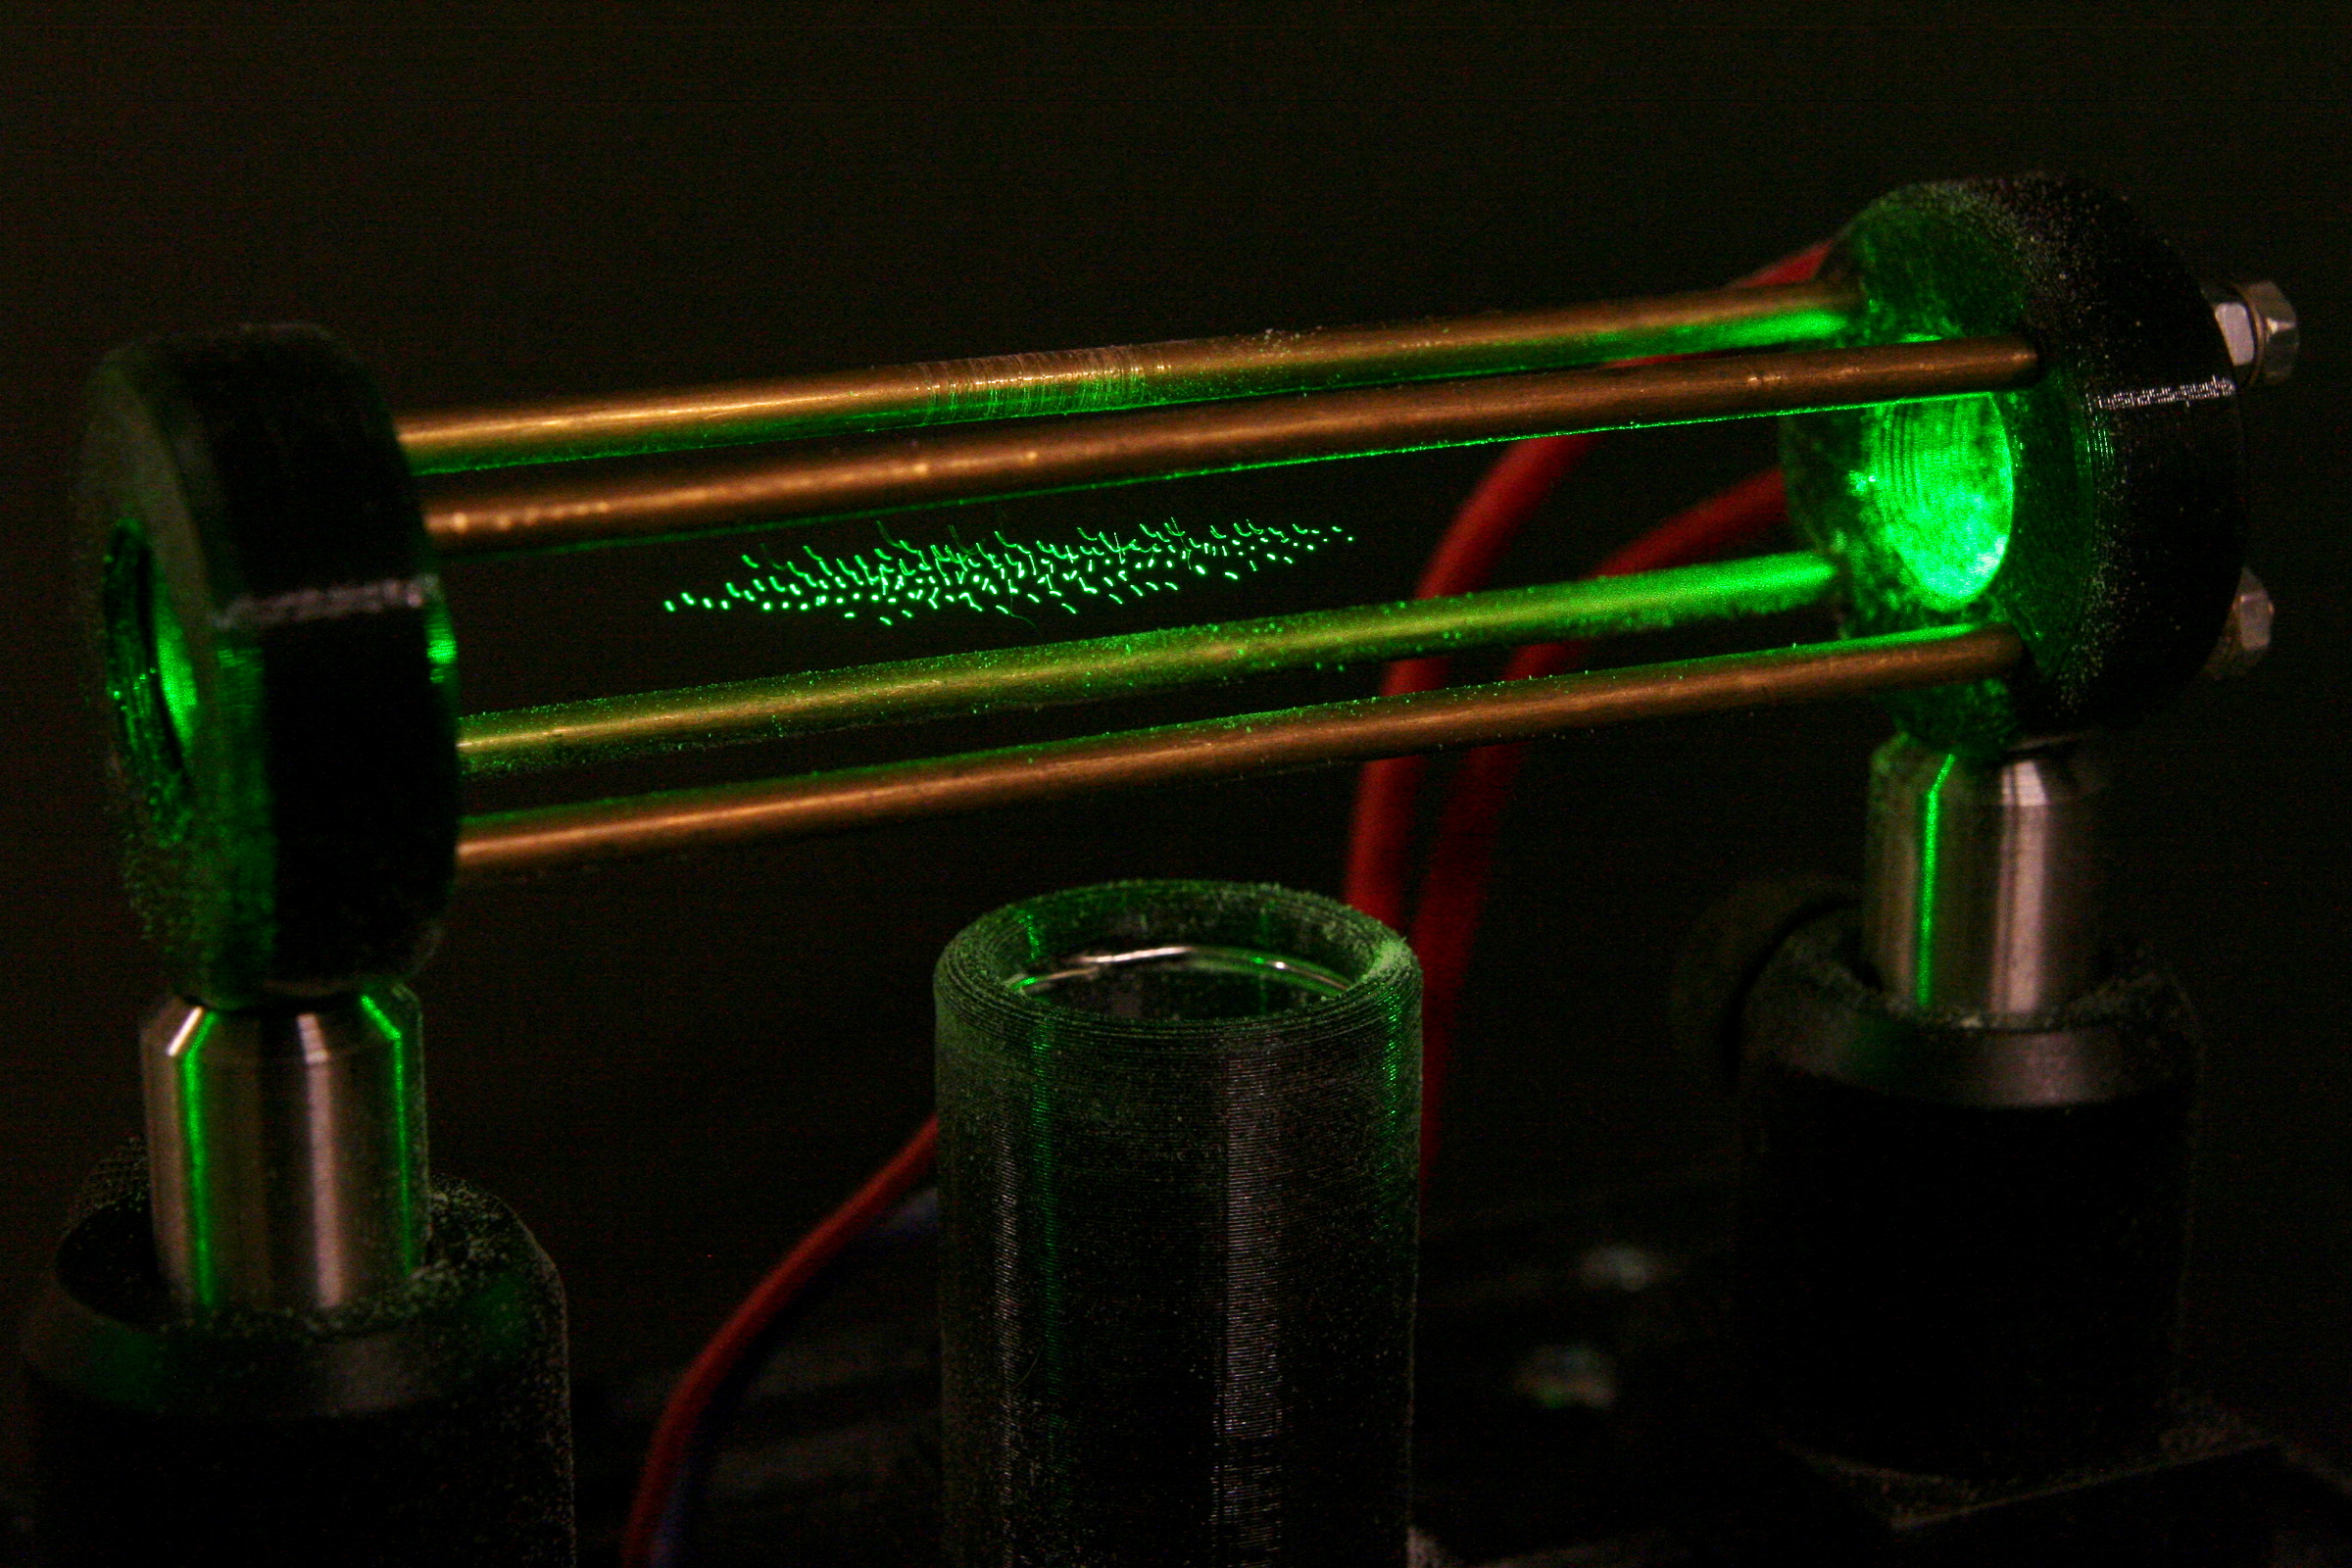
\includegraphics[width=0.9\textwidth]{images/ITQC_RFQ_Flour.jpg}
    \caption{Charged flour grains trapped in a simple Paul trap, the mentioned 4 parallel rods are visible and the electrodes creating the potential well are in the end caps.(**cite Pavelka, found on wikipedia)}\label{fig:ITQC_RFQ_Flour}
\end{figure}

\subsubsection{Notes on Other Paul Trap Designs}
Firstly, the aforementioned simple Paul trap was a linear Paul trap, in this type of Paul traps the ion's motion is confined in 2 dimensions by an RF quadrupole and the last is taken care of using a linear static potential, this is the type of trap on which we will focus.
There are also point Paul traps, which utilise oscillating RF fields for trapping in all 3 dimensions, these are also used for quantum computing, however when multiple ions are trapped together (which is necessary for entanglement) their motion is significantly more complex.

With focus on linear Paul traps there is still a plethora of different designs, most notably there are "surface" Paul traps.
These are usually microfabricated plates with a layout of electrodes on their surface which when driven by the correct voltages give rise to the same fields as the aforementioned simple linear Paul trap above their surface.
These designs offer great advantages for quantum computing, as not only are they cheaper and quicker to manufacture, but can be produced with a much higher precision than manually assembled devices.
In addition, they also have the benefit of the trapped ions being much more accessible for manipulation through lasers, in fact 



% There are many different ways of constructing a Paul trap, different electrode geometries give different benefits and downsides.

% For quantum computing we are mainly interested to trap individual ions in a predictable and stable way, there are 2 main types of ions traps that are used, the Penning tr


\section{Notes on Entanglement and error correction}
\subsection{Entanglement}
\subsubsection{What is Quantum Entanglement (basic idea)?}

\subsubsection{Local Realism}
Local Realism is the combined principle of Locality and Realism.
\vspace{1em}

\textbf{What is Locality}

Locality is the principle which essentially states that objects can only be acted upon by the 'local' (or surrounding) space around it. So by locality, a particle at some far distance can only be acted upon by us if something such as an EM field travels through the medium between us to get to it.
\vspace{1em}

\textbf{What is Realism}

This principle refers to the existence of a pre-existing property that has a definite value within a particle, wave-function or object before you measure said property and can determine what value that is. It can be likened to the classic 'tree in an abandoned forest' thought experiment where realism assumes that the tree always exists in a specific state of upright or fallen despite your lack of knowledge of that state.
\vspace{1em}

\subsubsection{Bell States \& the Bell Inequality}
The reason why local realism is important is because the famous EPR paper which argues that our current understanding of quantum mechanics is incomplete (due to the phenomenon of quantum entanglement) assumes that local realism must be observed which John Bell in 1964 goes on to prove is an assumption not upheld in quantum mechanics. \\

The CHSH inequality is as follows:
\begin{itemize}
    \item Victor prepares 2 particles for Alice and Bob who are at some large distance from each other(large enough that they cannot communicate before the particles reach them), each will get one of the two particles
    \item Alice can decide to measure one of two properties on her particle with the measurements themselves being $A_{0}$ or $A_{1}$. These properties, once measured, can hold the values $a_{0}$ and $a_{1}$ respectively; both of these values can be $\pm 1$.  
    \item Bob can do the same with his measurements being denoted as $B_{0}$and $B_{1}$ and the values they can take being $b_{0}$ and $b_{1}$ respectively. And just the same $b_{0,1} = \pm 1$
    \item We're now going to perform a somewhat arbitrary sum where we go over all the possible combinations of values that can be measured: 
    \begin{equation}
    a_{0}b_{0} + a_{0}b_{1} + a_{1}b_{0} - a_{1}b_{1}
    \end{equation}
    This can be factorised to: 
    \begin{equation} \label{CHSH classical sum}
        (a_{0} + a_{1})b_{0} + (a_{0} - a_{1})b_{1}
    \end{equation}
    \item Since $a_{0}$ and $a_{1}$ can only = $\pm 1$ then $a_{0} = a_{1}$ or $a_{0} = -a_{1}$ so then looking at (\ref{CHSH classical sum}) we can see that either the $b_{0}$ term will vanish or the $b_{1}$ will
    \item The important takeaway from this is that (\ref{CHSH classical sum}) = $\pm 2$ and now we're going to calculate the average value of (\ref{CHSH classical sum}) by having Victor send many particles (two at a time, one to each of them, per trial) and having Alice and Bob measure each of these.
    \item Due to the fact that Alice and Bob can only perform one measurement at a time, (\ref{CHSH classical sum}) cannot be deduced in one singular trial but we'll assume that the underlying properties exist and then we'll take an average of each term to determine the average value of (\ref{CHSH classical sum}) over many trials
    \item This then gives what we call a Bell inequality:
    \begin{equation} \label{CHSH inequality}
        \langle A_{0}B_{0} \rangle + \langle A_{0}B_{1} \rangle + \langle A_{1}B_{0} \rangle- \langle A_{1}B_{1}\rangle \leq 2
    \end{equation}
\end{itemize}

The Bell inequality derived above shows that assuming locality (that Alice and Bob cannot communicate to each other through super-luminal methods) and realism (that the properties $a_{0}$, $a_{1}$, $b_{0}$ and $b_{1}$ exist without having to apply a measurement \textit{or measurement operator} such that you can take the averages of $A_{0}$, $A_{1}$, $B_{0}$ and $B_{1}$) without actually applying them to their respective particles) there is an upper bound with which the average of (\ref{CHSH classical sum}) can take and that is 2.

\vspace{1em}

We will show that taking Quantum Mechanics into account, we can reach an upper bound of $2\sqrt{2}$ which means that one (or both) of the two assumptions of Locality and Realism is not observed in Quantum Mechanics. This implies that Quantum Entanglement is not the result of some incomplete part of Quantum Mechanics (as suggested in the EPR paper) but rather a phenomena that just doesn't observe local realism.

Proof Using Bell States and Pauli Gates:
\begin{itemize}
    \item Victor send a pair of qubits to Alice and Bob and prepares them in the Bell State (\ref{Bell state Definition}).....
\end{itemize}

\subsubsection{How to perform Quantum Entanglement on a QC}
There are many ways to perform QE in a quantum circuit but the easiest and simplest methods create the maximally\footnote{When we say 'maximally entangled' we mean that the entangled state can be written as a sum of pure states and a pure state is one in which we have exact information about (such as $|0\rangle$). Beware of the fact that whilst this does mean we have information about the entangled state as a whole, we cannot say the same about the individual qubits/subsystems/bases that make that entangled state.} entangled states known as bell states \label{Bell state Definition}. One such way involves taking a 2-qubit circuit or state and performing a Hadamard Gate Operator on the first qubit, proceeding this you perform a Controlled-Not Gate Operator across the 2 qubits with the control being the first qubit and the target being the second. This then produces the Bell state $\frac{1}{\sqrt{2}}(|00\rangle + |11\rangle)$

%Matrix operation Math




\subsubsection{Using Quantum Entanglement}
\begin{itemize}
    \item Superdense coding
    \item Quantum Teleportation
    \item Quantum Key Distribution
\end{itemize}



\subsection{Error Correction}
\begin{itemize}
    \item Bit and Sign Flip
    \item Shor Code
    \item Toric Codes
\end{itemize}
\subsection{Notes on Topological Quantum Computers}
Several pairs of non-abelian anyons are created. These anyons can be compared to Majorna Zero Modes (MZM) (which are constructs that allow fermions to be described as two seperate halves). Individual anyons when locally observed are indistinguishable in their ground states but when you look at the entire system and swap two anyon positions then the wave function that describes the system changes. The action of swapping two anyons can be described by a 'braid' matrix that transforms the wave function. The idea of braiding anyons is important because unlike Bosons and Fermions whose wave functions remain the exact same after you swap two of them around each other twice, the anyon wave function keeps a count of how many times they were swapped (or rather, braided)
A QC can be built up by creating pairs of anyons (initialising your qubits), treating the braid matrices as different gate operators (depending on which anyons are swapped) and then bringing pairs of anyons together (effectively taking a measurement) and seeing which anyons annihilate completely and which ones release a fermion (the fermion produced from the two halves of the MZM.\\
\textit{Important note: Abelian anyons were first detected in 2020, Non-abelian anyons are yet to be detected but are an active area of experiment and research}

\section{Pablo's notes}

To effectively perform quantum computation it is necessary to be able to manipulate qubits and perform unitary operations on them. Furthermore, any unitary transformation can be composed of single qubit operations and CNOT gates. Thus, an experimental quantum computer should be able to implement them appropriately.

\subsection{Optical Photon Quantum Computer}

The correct combination of phase shifters and beam splitters allow the creation of any single qubit gate. This is a consequence of the theorem that states that any single qubit operation can be generated from z and y-axis rotations. A phase shifter performs $R_{z}$ rotations and a beamsplitter performs $R_{y}$ rotations.

Nonlinear Kerr media allow for the creation of a two qubit gate. The main experimental problem with this setup is succesfully making two photons interact. The available nonlinear Kerr media today cannot reliably obtain the $\pi$ cross phase modulation necessary to implement a CNOT gate. 

\subsection{Optical cavity quantum electrodynamics}

The main idea behind this model is the question of whether the state of a photon can be transferred to and from single atoms, whose interactions would be easier to control. Single qubit operations are constructed in the same way as in the optical photon quantum computer.

The CNOT gate can be implemented by coupling atoms enclosed in a Fabry-Perot cavity to the optical field of the photons.

\subsection{Ion Trap}

Have to talk it over. Have not managed to fully understand how quantum gates would be constructed in this setup.

\subsection{Nuclear Magnetic Resonance}

The main difference with this method compared to the previous is that we are acting on an ensemble of particles. Arbitrary single qubit transforms can be constructed from magnetic field pulses applied to spins in a strong magnetic field. Coupling between the molecules and, thus, the realization of a two qubit gate can be provided by chemical bonds between neighbouring atoms.

\section{Matthew's notes}

\subsection{What are registers?}
Registers are a form of memory for data instantaneously in use by the CPU (https://www.javatpoint.com/computer-registers). Any data that the CPU wants to process must first be stored in a register. Fundamentally, a register is a group of flip-flops which can each store a bit of data. 

Give an example of a register..
Explain what a flip flop is..

\subsection{Quantum Registers}
Quantum registers are analogous to classical registers because they store the data that is processed by the computer. 

Rather than a group of flip-flop circuits, it is a superposition of qubits. A classical register can store one of $2^n$ different values for $n$ flip-flops. By comparison, a quantum register of $n$ qubits can store all $2^n$ values simultaneously (https://cds.cern.ch/record/383367/files/p165.pdf). A quantum computer will require multiple registers for true computation (https://arxiv.org/pdf/quant-ph/9802065), for example by adding the contents of two registers together.

\subsection{Why use QCs?}
Originally proposed by Richard Feynman to solve quantum mechanics problems, these computers will be useful for molecular simulation which can be used for drug development. Particularly good for financial calculations which involve a lot of combinatorics (https://epjquantumtechnology.springeropen.com/articles/10.1140/epjqt/s40507-021-00091-1). Financial institutions will also be able to afford high investment into QC development. Typical programs use Monte Carlo simulation of market movements. Goldman Sachs is one example

\begin{itemize}

\item Explain why combinatorics problems are easily solved
\item Could talk more about Monte Carlo
\item Weather forecasting
\item https://learn.microsoft.com/en-us/azure/quantum/concepts-overview
\item https://medium.com/@markus.c.braun/a-brief-history-of-quantum-computing-a5babea5d0bd
\end{itemize}
Quantum computers have the potential to break much of today's encryption, particularly RSA which is based on prime factorisation. However, they also open the door to modern cryptography, such as quantum key distribution (QKD) which is theoretically unbreakable by laws of Physics rather than just mathematically difficult to solve.

\subsection{Why not to use QCs}
Although quantum computers have the potential to allow for many of the breakthroughs described above, they will not replace classical ones. Instead, both systems are likely to coexist. Many of the things that an average user uses a computer for could not be enhanced to for any practical benefit by a quantum computer. There is some classical computation that could in fact be much slower on a quantum machine due to all the extra overheads required to run one. Streaming video or writing documents involves a certainty in the data, if you press a key on the keyboard there is no ambiguity in what to store that as internally. Therefore, there is no need to consider all possibilities when doing day to day computation (https://ieeexplore.ieee.org/stamp/stamp.jsp?tp=&arnumber=8322045).

\subsection{Major Breakthroughs}
\begin{itemize}
    \item 1998 - first demonstration of two qubit system (https://semanticscholar.org/paper/6c055053f4f1605fdc0bd474c7a350dcd01f627d)
    \item 2019 - google declares quantum supremacy by performing a series of operations in 200 seconds that would take a supercomputer about 10,000 years to complete; IBM responds by suggesting it could take 2.5 days instead of 10,000 years, highlighting techniques a supercomputer may use to maximize computing speed (https://www.forbes.com/sites/gilpress/2021/05/18/27-milestones-in-the-history-of-quantum-computing/?sh=2506dc67b23f)
    \item 2021, IBM eagle which is 127 bit quantum processor. First QC which is so complex that it cannot be simulated reliably by a classical computer 'the number of classical bits necessary to represent a state on the 127-qubit processor exceeds the total number of atoms in the more than 7.5 billion people alive today' (https://newsroom.ibm.com/2021-11-16-IBM-Unveils-Breakthrough-127-Qubit-Quantum-Processor)
\end{itemize}


\section{Superconducting QC stuff}

\begin{itemize}
    \item Currently used by Google, IBM, etc. and other big companies
    \item Cooper pairs are formed when an electron moves through a lattice, it pulls positive ions in the lattice closer to it as it moves along, creating a 'ripple' effect of increasing positive charge distribution, which then attracts nearby electrons to the ripple and forms a couple with the first electron. These electrons are paired and are called Cooper pairs. Their mutual repulsion keeps them away from each other and propels one when the other gets too close, and the other is pulled to the first when the first one creates a denser positive charge distribution. This way they propel each other without force and form superconducting electrons. 
    \item 3 types – Flux, Charge, Phase
    \item Most helpful \url{https://pennylane.ai/qml/demos/tutorial_sc_qubits.html}
    \item DVC1 : Very scalable because Josephson junctions are made on chips with 'easy' manufacturing techniques, however since the principle is having quantum effects on macroscopic level, too much scaling has issues with losing some quantum properties.
    \item DVC2 : Easily satisfied, because "Since the excited states in an artificial atom are short-lived and prefer to be on the ground state, all we have to do is wait for a short period. If the circuit is well isolated, it is guaranteed that all the qubits will be in the ground state with a high probability after this short interval." from PennyLane
    \item DVC3 : Hard because qubits are short-lived
    \item DVC4 : Somewhat challenging, currently done using 'capacitative coupling', however WiKipedia Superconducting QC page says doable
    \item DVC5 : easily doable by shining specific frequency light that brings excited state to
    \item 
    \url{https://jonathan-hui.medium.com/qc-how-to-build-a-quantum-computer-with-superconducting-circuit-4c30b1b296cd}
    \item 
    \url{https://www.reddit.com/r/askscience/comments/h0t51/comment/c1rr48v/?utm_source=share&utm_medium=web2x&context=3}
    \item \url{https://quantum.phys.cmu.edu/QCQI/QC_CMU2}
    \item \url{https://www.nature.com/articles/s41586-019-1666-5}
    \item \url{https://www.nature.com/articles/nature07128#Sec1}
    \item \url{https://www.nature.com/articles/s41534-016-0004-0#Sec2}

\end{itemize}

\section{Linear Optical Quantum Computing}\label{sec:Photonic}
Trapped ion quantum computing has made significant practical advances, however, the fundamental concepts of qubits and entanglement aren't limited to any one particular implementation but rather revolve around a quantum system (or systems). Therefore, this section explores a method using photons to represent qubits and then performs operations on those photons to implement quantum logic gate operations on qubits. Linear Optical Quantum Computing (LOQC) is the name used for photonic quantum computers that make use of classical linear optical tools such as beamsplitters, polarisers, phase shifters, etc. to perform these operations. What makes LOQC's so interesting to explore is the unique way some problems such as scalability is challenged but we will cover that later in this section. The first step is to transform photons into qubits.

\subsection{Types of Encoding}
The ways in which a photon can be made to represent a qubit is known as the method of "encoding". Much like the different methods for quantum computing in general, there are many different ways to encode photons to represent qubit states; there exists mixed polarisation encoding, parity encoding etc. For this report will focus on spacial encoding, specifically dual-rail encoding. 

\subsubsection{Spacial Modes}\label{sec:modes}
Single rail encoding involves sending a photon down a single rail or cavity; imagine a photon traveling down a wire. The existence of a photon in the rail is representative of a qubit with state $\ket{1}$, whilst nothing but vacuum in the rail is representative of a qubit in state $\ket{0}$. Dual rail encoding is very similar but instead of a single rail/cavity, there are two. In this case, the rails (sometimes called modes) can be labeled A and B; when a photon is detected in mode A but not B this is representative of a qubit with the state $\ket{0}$. When a photon is detected in mode B but not A this is representative of a quibt with the state $\ket{1}$. 

What is the difference between these types of encoding? As it turns out, performing 2 qubit gate operations (and then entangling multiple qubits) in a single rail encoded quantum computer is very simple; it involves the use of a linear optical tool called the beamsplitter and the phenomena known as the Hong-Ou-Mandel effect \cite{PhysRevLett.59.2044}(both of these are discussed in more detail later). However, in a dual-rail representation achieving this deterministically isn't physically possible. Similarly, in the dual rail representation, performing 1 qubit operations is quite simple but it is not physically possible to achieve deterministically in the single rail representation. The rest of this section will have a heavy focus on the dual-rail representation and discuss how non-deterministic, or rather probabilistic, tools are used to create 2 qubit gate operations. It is important to note that mathematically, the horizontal-vertical polarisation representation, as introduced in \cref{sec:superposition}, is identical to the dual rail representation. 


%%%%%%%%%%%%%%%%%%%%%%%%%%%%%%%%%%%%%%%%%%

\subsection{Useful Linear Optical Tools and Single Qubit Representations}
Before going into any of the complex techniques that really support photonic quantum computers as a viable, scalable direction for quantum computers of the future, the report will introduce some of the basic tools that can manipulate photons and by extension, qubits.
\subsubsection{Beamsplitters}

The aptly named beamsplitter divides a beam of light into two. The intensity of each outgoing beam is determined by the angle at which the beamsplitter is placed relative to the incoming beam. The type of encoding used affects the design of the beamsplitter. In dual rail encoding, two glass prisms are placed back to back and a half-silvered mirror is placed between them \cite{nielsen_chuang_2010}. %place image of this from QC&QI

When applied to a qubit, the action of the beamsplitter is equivalent to performing a transformation on the qubit's state, which can be represented as $B_{\theta\phi} = $ $\begin{bmatrix}
cos(\theta) & -e^{i\phi}sin(\theta) \\
e^{-i\phi}sin(\theta) & cos(\theta) 
\end{bmatrix}$. \cite{KnillE2001Asfe} Here, $\theta$ determines the transmission and reflection amplitudes of the outgoing beams, the reflection amplitude R= $sin^2(\theta)$ and the transmission amplitude T = 1-R = $cos^2(\theta)$), and $\phi$ is the phase shift applied by the beamsplitter.

\subsubsection{Phase Shifters}
Phase shifters are a simple yet effective tool in quantum computing. To use them, one employs a material with a higher refractive index than the medium the photons are passing through (such as air), and guides the beams through this material to induce a phase shift \cite{nielsen_chuang_2010}. 

The phase shifter performs a transformation on the qubit, described as $P_\phi = $ $\begin{bmatrix}
1 & 0 \\
0 & e^{i\phi}
\end{bmatrix}$, where the phase shift $\phi$ is given by the thickness and refractive index of the phase shifter. It's worth noting that, when $\phi = \frac{\pi}{2}$, the phase shift gate is equivalent to the Pauli Z transformation. This is valid for all phase shift gates, not just the optical one mentioned here.

\subsubsection{Mirror}
A mirror is a step further towards simplicity from the tools listed before as it simply reflects beams with near 100\% intensity. We can describe the action of a mirror on a photonic qubit as a special case of the beamsplitter where the reflection intensity is 100\% and the phase shift $\phi = 0$  \cite{nielsen_chuang_2010}.

\subsubsection{Photodetectors}
A photodetector detects the arrival of photons. It accomplishes this by converting the energy deposited by the photon onto its surface into an electrical signal which can be measured and quantified. The quantum efficiency $\eta$ of a photodetector is the probability that a single incident photon generates an electrical signal that contributes to the overall detector current. This component is crucial in an optical quantum computer as it allows the readout of the output of the quantum computer \cite{nielsen_chuang_2010}. 


\subsubsection{Nonlinear Kerr Media}
As we will cover in the next section, in Linear Optical Quantum Computing, deterministic processes can only take us so far. What we mean by this is that when we want to employ phenomena such as entanglement, it is impossible to accurately entangle our qubits all the time with a 100\% success rate only using the tools we have listed above (deterministic, predictable tools). To get around this we can either use probabilistic (non-deterministic) qubit gates or Kerr media. Kerr media are physical materials that have a non-linear refractive index, these refractive indices may vary with the intensity of the incident photon beam and so a photon beam with a larger intensity will experience a greater phase shift as a result of a greater refractive index.

In Linear Optical Quantum Computing, deterministic methods alone can have limitations in generating entanglement between qubits as we will cover in the next section. However, it is possible to achieve high success rates for entanglement  by employing other techniques or materials alongside the linear optical elements. One such material is nonlinear Kerr media, which have a non-linear refractive index, meaning that the amount of phase shift experienced by an incident photon beam is dependent on the intensity of the beam \cite{nielsen_chuang_2010}. The refractive index of the material increases with the intensity of the incident beam, leading to a greater phase shift for a photon beam with a larger intensity. Additionally, there are also probabilistic methods, such as the KLM protocol, which will be covered in Section 4.5 of the report.



\par 
The most important property of a Kerr medium is the cross-phase modulation it provides. For a two qubit state expressed in single rail encoding, Kerr media have the following effect:
%For a two-qubit register, Kerr media have the following effect:

\begin{align*} 
    K \ket{00} &=  \ket{00}\\
    K \ket{01} &=  \ket{01}\\
    K \ket{10} &=  \ket{10}\\
    K \ket{11} &=  e^{i\chi L}\ket{11}
    \end{align*}
    
If the cross-phase modulation $\chi L$ is taken to be $\pi$, then $K \ket{11} =  -\ket{11}$. This can be expressed as a matrix K acting on two qubits.

$$K = \begin{bmatrix}
    1 & 0 & 0 & 0\\
    0 & 1 & 0 & 0\\
    0 & 0 & 1 & 0\\
    0 & 0 & 0 & -1\\
    \end{bmatrix}$$

If the matrix K was then left and right multiplied by the Hadamard gate acting individually on both qubits, a C-NOT gate could be constructed. 

The main issue with nonlinear Kerr media is the difficulty of producing a material with a high cross phase modulation ratio without incurring substantial losses due to absorption. It is theoretically estimated that, in the best possible case, approximately 50 photons must be absorbed for each photon which experiences a $\pi$ phase modulation, as stated in section of 7.4.2 of \cite{nielsen_chuang_2010}. Thus, if this were the only method to entangle photons, a single photon quantum computer would be extremely hard to physically construct.



%%%%%%%%%%%%%%%%%%%%%%%%%%%%%%%%%%%%%%%%%%



%%%%%%%%%%%%%%%%%%%%%%%%%%%%%%%%%%%%%%%%%%%

\subsection{Two Qubit Operations}
Now that we have looked at all of our linear optical tools that are used to create one qubit gates in our dual representation, we can start to look at how 2 qubit gates are implemented but there's a problem. We touched on this slightly in the previous section about the Kerr effect but it is actually impossible to implement a completely deterministic 2-qubit gate operation in the dual rail model\cite{PhysRevA.59.3295}\cite{PhysRevA.62.064301}. We can see this in more detail when we consider the example of making a maximally entangled Bell state \footnote{We mentioned bell states in  \cref{eqn:entqubit} but we cover them in more detail in \ref{eqn:Bell States}.}. Below is the kind of transformation we hope to achieve, transforming a state such as $\ket{0,0}$ into the maximally entangled Bell state.
\begin{equation} \label{bob bell state}
    \ket{0,0} \rightarrow \frac{1}{\sqrt{2}}(\ket{0,1} + \ket{1,0})
\end{equation}

The circuit that is supposed to create the bell state on the right-hand side above is decribed by the following transformation:
\begin{equation} \label{bogoliubov}
    \hat{a}^{\dag}_{\color{red}0}\hat{b}^{\dag}_{\color{red}0} \rightarrow (\sum\limits_{k={\color{red}0},{\color{red}1}}\alpha_k\hat{a}^{\dag}_k + \beta_k\hat{b}^{\dag}_k)(\sum\limits_{k={\color{red}0},{\color{red}1}}\gamma_k\hat{a}^{\dag}_k + \delta_k\hat{b}^{\dag}_k)
\end{equation} \cite{Kok:2005jip}
where $\hat{a}^\dag_{\color{red}0}$ is the creation operator acting on the zeroth mode \footnote{the ${\color{red}0}$ subscript signifies the operator acting on the zeroth mode} of the first qubit (creating the state $\ket{0}$ in the first qubit); $\hat{b}^\dag_{\color{red}0}$ is the creation operator acting on the zeroth mode of the second qubit; $\alpha, \beta, \gamma$ and $\delta$ are constants that can be varied.
\par
No matter how we vary the constants,  $\alpha, \beta, \gamma$ and $\delta$, the right-hand side of \cref{bogoliubov} can be (and is) separated in terms of each qubit where Bell states and entangle qubits cannot:
\begin{equation}
    (\sum\limits_{k={\color{red}0},{\color{red}1}}\alpha_k\hat{a}^{\dag}_k + \beta_k\hat{b}^{\dag}_k)(\sum\limits_{k={\color{red}0},{\color{red}1}}\gamma_k\hat{a}^{\dag}_k + \delta_k\hat{b}^{\dag}_k) \neq \hat{a}^{\dag}_{\color{red}0}\hat{b}^{\dag}_{\color{red}1} + \hat{a}^{\dag}_{\color{red}1}\hat{b}^{\dag}_{\color{red}0}
\end{equation}
The right-hand side represents the creation operators that, when applied to a vacuum state, create the Bell state seen in \cref{bob bell state}.

It should be noted that this problem is not limited to dual rail encoding, in single rail encoding it is equally as hard to create single qubit gates but implementing two-qubit gates is as simple as using linear optical tools.

To work around the problem we have in creating two-qubit gates one could implement the use of Kerr media as discussed above, however in this report, we will focus on probabilistic gate methods below.


\subsubsection{Control-Z gate (Control Phase Shift Gate)}
The Hong-Ou-Mandel (HOM) \cite{PhysRevLett.59.2044} effect was mentioned previously in \cref{sec:modes}. This is an interesting phenomenon that plays a pivotal role in optical quantum computing. Imagine two photons enter a 50:50 beamsplitter from modes A and B which can be written as $\ket{1,1}_{a,b}$. This state can be considered in terms of the creation operators $\hat{a}^\dagger$ (acting on A) and $\hat{b}^\dagger$ (acting on B) in the following way $\hat{a}^\dagger\hat{b}^\dagger\ket{0,0}_{a,b}$. When the photons exit the beamsplitter there is a 50:50 chance that the photons could come out through rail C or rail D. Therefore, by going through the beamsplitter, the state $\hat{a}^\dagger\hat{b}^\dagger\ket{0,0}_{a,b}$ is transformed into $\frac{1}{2}((\hat{c}^\dagger)^2 - (\hat{d}^\dagger)^2)\ket{0,0}_{c,d}$ \footnote{ the beamsplitter transforms $\hat{a}^\dagger\ket{0}_a$ into the state $\frac{1}{\sqrt{2}}(\hat{c}^\dagger + \hat{d}^\dagger)\ket{0}_c$ whilst transforming  $\hat{b}^\dagger\ket{0}_b$ into the state $\frac{1}{\sqrt{2}}(\hat{c}^\dagger - \hat{d}^\dagger)\ket{0}_c$. Physically this can be described as the photon from rail B being phase shifted by $\pi$ when reflected from the beamsplitter and going into rail D}. This is important because, recalling that $\hat{a}^\dagger, \hat{b}^\dagger, \hat{c}^\dagger$ and $\hat{d}^\dagger$ are creation operators, this is equivalent to $\frac{1}{\sqrt{2}}(\ket{2,0}_{c,d} - \ket{0,2}_{c,d})$.

In words, when 2 photons coming from different rails enter into a 50:50 beamsplitter at the same time on separate rails A and B, they will both exit on the same rail, C or D. This can be described as photon bunching but it is formally known as the Hong-Ou-Mandel effect and "lies at the heart of linear optical quantum computing" \cite{Kok:2005jip}

As stated earlier, implementing two-qubit gates must have some probabilistic, non-deterministic element to them and to achieve this we will be using the non-deterministic phase shift gates which we'll cover in more detail in the next section but the important thing to note now is that when looking at the 3 lowest Fock states, these NS gates phase flip the 3rd lowest:
\begin{equation} \label{NS evolution}
    \alpha\ket{0} + \beta\ket{1} + \gamma\ket{2} \rightarrow \alpha\ket{0} + \beta\ket{1} - \gamma\ket{2}
\end{equation} \cite{Kok:2005jip}

\begin{figure}[h]
    \centering
    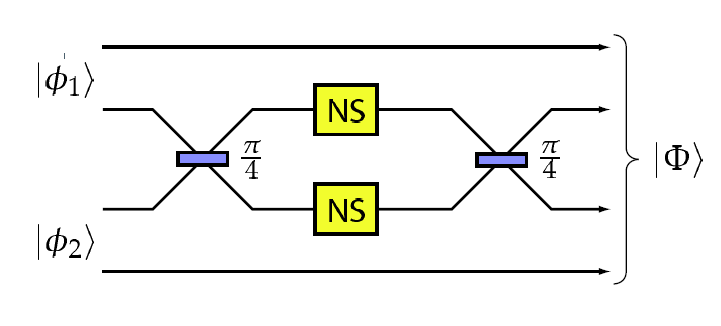
\includegraphics[width=0.9\textwidth]{images/CZ-gate.png}
    \caption{Circuit for the Control-Z gate which applies a phase shift of $\pi$ to the qubit $\ket{\phi_2}$ if (and only if) both qubits are in the state $\ket{1}$. The modes for each qubit above are reversed such that a state of $\ket{11}_{\phi_1\phi_2}$ means that the middle 2 modes are populated by a photon. The blue rectangles in this diagram represent beamsplitters at the angle $\frac{\pi}{4}$. figure taken from \cite{Kok:2005jip}}\label{fig:CZ_gate}
\end{figure}

As we can see in \cref{fig:CZ_gate}, when $\ket{\phi_1}$ and $\ket{\phi_2}$ are both equal to $\ket{1}$ then there will be a photon in the middle two modes ($\ket{\phi_2}$ is flipped). This means that the two photons will interact at the first beamsplitter, via the Hong-Ou-Mandel effect they will "bunch" and go down the same mode together towards the NS gate. The NS gate will sign flip the photons in the mode they went down due to the NS evolution \cref{NS evolution} and then the photons will interact with the second beamsplitter to finally give the state $-\ket{1,1}$.%\textbf{EVERYTHING AFTER THIS IS WRONG} What makes this circuit interesting is that because of the HOM effect, this situation only occurs when $\ket{\phi_1}$ and $\ket{\phi_2}$ are both equal to $\ket{1}$. In the case where only one photon goes through the middle modes, the photon will be split by the beamsplitter into both modes, each mode will interact with the NS gate, acquiring a phase shift each but these phase shifts destructively cancel when the modes are brought together at the second beamsplitter and the HOM effect occurs again. Due to the fact that the NS gate has a 1/4th probability of operating correctly and this gate requires two in tandem, the probability of the CZ gate operating as we expect is $p_{CZ} = p_{NS}^2 $

\subsubsection{Nonlinear phase shift gate}
As stated above, the nonlinear phase shift gate is a very useful tool as its non-deterministic effects allow us to achieve maximally entangled states when we otherwise couldn't but how is the NS gate made? The circuit is actually fairly simple; it involves 2 ancillary modes, one with a photon present and the other without, 3 beamsplitters set at differing angles with no phase shift and then 2 "perfect" photon detectors. We can see this in \cref{fig:NS_gate}. Going through each case for this NS gate is quite exhaustive which we won't cover here but the important thing to note is that 1/4 of the time the fock states $\alpha\ket{0}$ and $\beta\ket{1}$ are left untouched and when two photons come through from $\phi$, $\gamma\ket{2} \rightarrow -\gamma\ket{2}$ 

\begin{figure}[H]
    \centering
    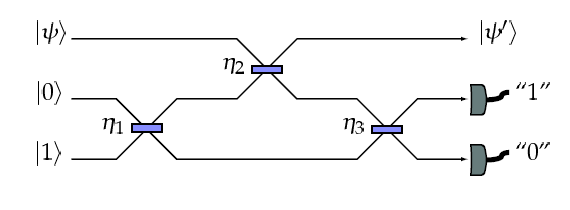
\includegraphics[width=0.9\textwidth]{images/NS gate.png}
    \caption{Circuit for the non-linear phase shift gate (NS) that applies a phase shift of variable amounts, typically a phase shift of $\pi$ which results in a sign flip (hence the other name, non-linear sign flip gate). 3 beamsplitters with varying angles are used as well as two 'ancillary' modes that we hope to detect as $\ket{1}$ and $\ket{0}$ respectively. If this doesn't happen then our NS gate has failed. figure taken from \cite{Kok:2005jip}}\label{fig:NS_gate}
\end{figure}
%%%%%%%%%%%%%%%%%%%%%%%%%%%%%%%%%%%%%%%%%%



\subsection{Efficiency}
As we know by now, the real magic of quantum computation occurs when we can implement two-qubit gates as this allows us to perform quantum entanglement between qubit states which is then instrumental in many other constructs such as Quantum Teleportation, Quantum Algorithms, etc.

The issue we tend to run across with LOQC is that photons tend to not naturally interact with each other. This makes the practical implementation of a two-qubit gate a very difficult task. One suggested method is to use nonlinear Kerr media to provide a cross-phase modulation of $\pi$ between photon states. This combined with a beamsplitter can be used to construct a CNOT gate, from which a universal set of gates can be obtained. However, as stated in Section 7.4.3 in \cite{nielsen_chuang_2010}, obtaining nonlinear Kerr media with sufficient cross-phase modulation is not possible without incurring an excessive absorption loss: for every photon that incurs a $\pi$ cross-phase modulation, approximately 50 photons must be absorbed. Another suggested method of overcoming this uses photo-detectors to make projective measurements which can induce an interaction between photons \cite{Kok:2005jip}. This is a probabilistic approach with the probability of success being rather small and the more probabilistic photo-detectors (or non-deterministic operations in general) that are used, the probability of success for the entire circuit decreases exponentially. This makes optical computation seem quite unfeasible on the large scale but thanks to a few interesting results in quantum optics we can implement what is referred to as the KLM protocol to construct scalable 2-qubit gates.

\subsection{Scalability and the KLM Protocol}
As you probably might have guessed by now, there is a major problem with photonic quantum computing as we've discussed that uses probabilistic gates and that is the fact that the probabilities of these gates are quite low. Having a CZ gate that only works 1/nth of the time means that to get some reasonable result we need to run our circuit n times. As we implement more complicated circuits that involve some number, n, of probabilistic gates with probabilities $\frac{1}{p}$, the chance of success of our circuit is $\frac{1}{p^n}$. This is obviously infeasible as any interesting circuit will require many gates and with our current set-up that means any scalable photonic quantum computer is too resource intensive to be worth it. \par
This alone sounds like it would be the nail in the coffin for further development into LOQC's but using quantum teleportation, the discrete quantum Fourier transform, and n number of photonic modes the probability of success for a given non-deterministic gate can become 'near-deterministic' with a success rate of $\frac{n^2}{(n+1)^2}$ which tends to 1 as n becomes sufficiently large. This is a process named the KLM protocol after Knill, Leflamme, and Milburn it was developed in 2000 and it is essential for any photonic quantum computer we could hope to build on a scale larger than a few gates.

\subsubsection{How does Quantum Teleportation work?}
Before we can get into how the KLM procedure works for near-deterministic photonic quantum computers we need to look at the phenomenon known as Quantum Teleportation. Unlike the name suggests, quantum teleportation does not involve 'teleporting' qubits in the common sense of the word; quantum teleportation is actually the process of transferring the exact state of one qubit to another. To expound upon this, quantum teleportation is the process of taking the initial state $\ket{\phi}_a = \alpha\ket{0} + \beta\ket{1}$ for some qubit \textit{a} and transferring it into some qubit \textit{b}. Quantum teleportation is limited in that information transfer (or in this case, 'teleportation') can not occur faster than light and due to the no-cloning theorem, the original qubit state is erased when being teleported to the second.
\par
We initially start with 2 entangled qubits being prepared by Eve. Eve then passes one of the entangled qubits to Alice and the other to Bob. Alice also has the initial qubit in state $\ket{\phi_j}$ that she wants to teleport it to Bob. Alice then performs a Bell Basis Measurement across her two qubits and then classically sends information about the outcome of that measurement to Bob. Bob then performs one of 4 computations to his qubit from Eve and after this Bob will have the state $\ket{\phi_j}$. Before any of this can happen though, Alice has to perform a Bell Basis Measurement. \\
We first saw Bell states in  \cref{eqn:entqubit} but there are a total 4 Bell states (or EPR pairs) that represent 4 sets of 2 maximally entangled qubits. These states are:
\begin{align}\label{eqn:Bell States}
    B_0 &= \frac{1}{\sqrt{2}}\ket{00} + \ket{11} \\
    B_1 &= \frac{1}{\sqrt{2}}\ket{10} + \ket{01} \\
    B_2 &= \frac{1}{\sqrt{2}}\ket{00} - \ket{11} \\
    B_3 &= \frac{1}{\sqrt{2}}\ket{10} - \ket{01} \\
\end{align} \cite{nielsen_chuang_2010}
where from here on out we'll omit the factor of $\frac{1}{\sqrt{2}}$ and the order of labeling of $B_n$ doesn't actually matter but we've chosen this way for simplicity. 
\par
A Bell Basis Measurement is what happens when we take an arbitrary 2 qubit state and project it onto one of the four bases listed above. As mentioned in \cref{sec:USoQG} this can be as simple as applying a Hadamard and a CNOT. So Alice takes her initial qubit $\ket{\phi_j} = \alpha\ket{0} + \beta\ket{1}$ and performs a Bell Basis Measurement over it with the entangled qubit received from Eve. Mathematically this looks like:
\begin{align} \label{eqn:Bells QT}
    (\ket{00} + \ket{11})(\alpha\ket{0} + \beta\ket{1}) = \alpha\ket{000} + \beta\ket{001} + \alpha\ket{110} + \beta\ket{111}
\end{align}
where in the above equation, the state $\ket{101}$ would mean Alice's 2 qubits are in the state $\ket{01}$ (the first being in 1 and the second being in 0) and Bobs is in $\ket{1}$. Remember that when reading the states of qubits we look from right to left. 

By performing the Bell Basis Measurement we project \cref{eqn:Bells QT} onto the states in \cref{eqn:Bell States}:
\begin{align}\label{eqn:final BM states}
    \alpha\ket{000} + \beta\ket{001} + \alpha\ket{110} + \beta\ket{111} = (\alpha\ket{0} + \beta\ket{1})B_0 + (\alpha\ket{1} + \beta\ket{0})B_1 \\ +(\alpha\ket{0} - \beta\ket{1})B_2 + (\alpha\ket{1} - \beta\ket{0})B_3 
\end{align}

We can see in \cref{eqn:final BM states}, when Alice looks at her qubits, if she sees $B_0$, the leftover state in Bob's qubit is $\alpha\ket{0} + \beta\ket{1} \equiv \ket{\phi_j}$. Teleportation has occurred and no further action is required. If Alice sees $B_1$ then the leftover state in Bob's qubit is $(\alpha\ket{1} + \beta\ket{0}) \equiv X\ket{\phi_j}$ where X represents the Pauli-X gate/ the quantum not gate operator $
\begin{bmatrix}
    0 & 1\\
    1 & 0\\
\end{bmatrix}$.If Alice sees $B_2$ then the leftover state in Bob's qubit is $(\alpha\ket{0} - \beta\ket{1}) \equiv Z\ket{\phi_j}$ where Z represents the Pauli Z gate (the Phase gate shown in \cref{eqn:phase} if $\phi = \pi$). Finally, if Alice sees $B_3$ then the leftover state in Bob's qubit is $(\alpha\ket{1} - \beta\ket{0}) \equiv ZX\ket{\phi_j}$. 

Since the Z and X gates are their own inverses, all Bob has to do is wait for Alice to communicate classically, which of the 4 states she observed and then apply the $\mathbb{I}$, X, Z or XZ gates to his qubit to get the initial qubit $\ket{\phi_j}$. This is all shown diagrammatically in \cref{fig:QT circuit}

\begin{figure}[h]
    \centering
    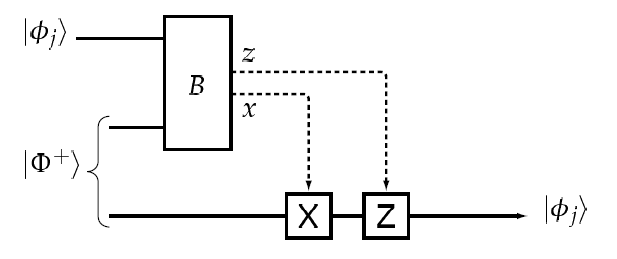
\includegraphics[width=0.9\textwidth]{images/QT circuit.png}
    \caption{Quantum teleportation circuit where the state $\phi_j$ is teleported to the second qubit. The bell measurement B gives one of 4 possibilities denoted $I, X, Z$, and $XZ$. The outcome is 'sent' classically (or in this case, we just measure what the outcome is) and then the corresponding gate is applied to the second qubit; the identity (nothing is done), the X gate (otherwise known as the not gate), the Z gate (otherwise known as the phase shifter), or the X followed by Z. figure taken from \cite{Kok:2005jip}}\label{fig:QT circuit}
\end{figure}

\subsubsection{How Teleportation can be used in CZ gates}
Now that we understand how quantum teleportation works in theory, we now want to implement this with our non-deterministic CZ gate to see if we can improve our probability of success.

The first thing we must note is that the CZ gate operates on two qubits and because our teleporter only outputs a single mode, we need to double the circuit in \cref{fig:QT circuit}, this looks like \cref{fig:QTCZ-1}. Now thanks to the fact that the CZ gate and the Pauli gates are in the Clifford group, we can commute the CZ gate with our X and Z gate operations \cite{GottesmanDaniel1999QTia}(with some corrections) to achieve a circuit that is identical to \cref{fig:QTCZ-1} in output. This looks like \cref{fig:QTCZ-2} where the dashed X and Z boxes represent applying some combination of X and Z gates depending on the outcomes of the Bell Measurement. There is a more comprehensive overview of this in the Appendix \ref{Appendix:A}. 

%##############################
\begin{figure}[H]
    \centering
\tikzset{every picture/.style={line width=0.75pt}} %set default line width to 0.75pt        

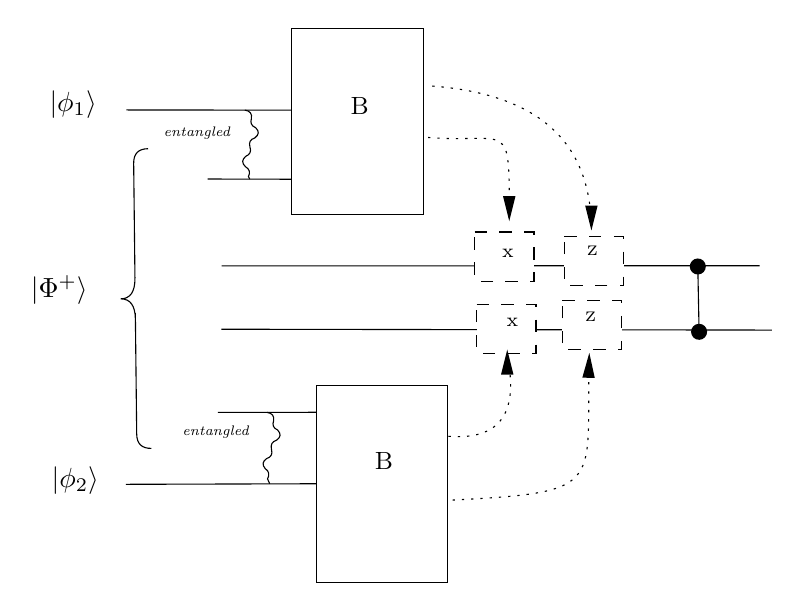
\begin{tikzpicture}[x=0.75pt,y=0.75pt,yscale=-1,xscale=1]
%uncomment if require: \path (0,300); %set diagram left start at 0, and has height of 300

%Shape: Brace [id:dp4160546662329181] 
\draw   (107.72,84.61) .. controls (103.05,84.66) and (100.75,87.02) .. (100.8,91.69) -- (101.42,146.88) .. controls (101.49,153.55) and (99.2,156.91) .. (94.53,156.96) .. controls (99.2,156.91) and (101.57,160.21) .. (101.64,166.88)(101.61,163.88) -- (102.26,222.08) .. controls (102.31,226.75) and (104.67,229.05) .. (109.34,229) ;
%Straight Lines [id:da8065384733259011] 
\draw    (97.23,65.94) -- (176.98,66.04) ;
%Shape: Rectangle [id:dp6790608484549128] 
\draw   (176.98,26.57) -- (240.39,26.57) -- (240.39,116.25) -- (176.98,116.25) -- cycle ;
%Straight Lines [id:da34073899408201536] 
\draw    (136.45,99.22) -- (176.98,99.32) ;
%Straight Lines [id:da3326977952142205] 
\draw    (97.07,246.31) -- (188.75,246.04) ;
%Shape: Rectangle [id:dp4807359036219334] 
\draw   (188.75,293.6) -- (252.15,293.6) -- (252.15,198.6) -- (188.75,198.6) -- cycle ;
%Straight Lines [id:da5430962616562778] 
\draw    (141.33,211.67) -- (188.75,211.61) ;
%Straight Lines [id:da9639318872173184] 
\draw    (143.18,141.07) -- (402.33,141) ;
%Straight Lines [id:da22467135117490433] 
\draw    (143.02,171.59) -- (408.33,172) ;
%Shape: Rectangle [id:dp5224143658365781] 
\draw  [fill={rgb, 255:red, 255; green, 255; blue, 255 }  ,fill opacity=1 ][dash pattern={on 4.5pt off 4.5pt}] (265.03,124.76) -- (293.66,124.76) -- (293.66,148.4) -- (265.03,148.4) -- cycle ;
%Shape: Rectangle [id:dp30201259432122174] 
\draw  [fill={rgb, 255:red, 255; green, 255; blue, 255 }  ,fill opacity=1 ][dash pattern={on 4.5pt off 4.5pt}] (307.38,157.82) -- (336.01,157.82) -- (336.01,181.45) -- (307.38,181.45) -- cycle ;
%Shape: Rectangle [id:dp20575966558705927] 
\draw  [fill={rgb, 255:red, 255; green, 255; blue, 255 }  ,fill opacity=1 ][dash pattern={on 4.5pt off 4.5pt}] (308.19,126.86) -- (336.82,126.86) -- (336.82,150.49) -- (308.19,150.49) -- cycle ;
%Shape: Rectangle [id:dp879155044923984] 
\draw  [fill={rgb, 255:red, 255; green, 255; blue, 255 }  ,fill opacity=1 ][dash pattern={on 4.5pt off 4.5pt}] (266.01,159.59) -- (294.64,159.59) -- (294.64,183.23) -- (266.01,183.23) -- cycle ;
%Curve Lines [id:da09246323435174553] 
\draw  [dash pattern={on 0.84pt off 2.51pt}]  (242.67,79.2) .. controls (282.34,82.32) and (281.78,68.69) .. (281.77,117.99) ;
\draw [shift={(281.76,119.5)}, rotate = 270] [fill={rgb, 255:red, 0; green, 0; blue, 0 }  ][line width=0.08]  [draw opacity=0] (12,-3) -- (0,0) -- (12,3) -- cycle    ;
%Curve Lines [id:da06959625459364571] 
\draw  [dash pattern={on 0.84pt off 2.51pt}]  (244.64,54.43) .. controls (284.31,57.55) and (320.6,72.61) .. (321.32,122.48) ;
\draw [shift={(321.33,124)}, rotate = 270] [fill={rgb, 255:red, 0; green, 0; blue, 0 }  ][line width=0.08]  [draw opacity=0] (12,-3) -- (0,0) -- (12,3) -- cycle    ;
%Curve Lines [id:da39316974650838654] 
\draw  [dash pattern={on 0.84pt off 2.51pt}]  (252.48,223.17) .. controls (289.95,226.11) and (282.09,193.82) .. (280.92,183.28) ;
\draw [shift={(280.78,181.42)}, rotate = 90] [fill={rgb, 255:red, 0; green, 0; blue, 0 }  ][line width=0.08]  [draw opacity=0] (12,-3) -- (0,0) -- (12,3) -- cycle    ;
%Curve Lines [id:da18722309143811278] 
\draw  [dash pattern={on 0.84pt off 2.51pt}]  (254.44,253.9) .. controls (329.57,250.04) and (318.6,247.3) .. (320.28,184.91) ;
\draw [shift={(320.33,183)}, rotate = 91.75] [fill={rgb, 255:red, 0; green, 0; blue, 0 }  ][line width=0.08]  [draw opacity=0] (12,-3) -- (0,0) -- (12,3) -- cycle    ;
%Straight Lines [id:da761825964657918] 
\draw    (372.6,141.36) -- (373.22,172.83) ;
\draw [shift={(373.22,172.83)}, rotate = 88.87] [color={rgb, 255:red, 0; green, 0; blue, 0 }  ][fill={rgb, 255:red, 0; green, 0; blue, 0 }  ][line width=0.75]      (0, 0) circle [x radius= 3.35, y radius= 3.35]   ;
\draw [shift={(372.6,141.36)}, rotate = 88.87] [color={rgb, 255:red, 0; green, 0; blue, 0 }  ][fill={rgb, 255:red, 0; green, 0; blue, 0 }  ][line width=0.75]      (0, 0) circle [x radius= 3.35, y radius= 3.35]   ;
%Curve Lines [id:da1435143281948974] 
\draw    (165.04,211.64) .. controls (167.55,212.01) and (168.61,213.36) .. (168.22,215.68) .. controls (167.48,217.79) and (168.12,219.27) .. (170.14,220.12) .. controls (171.89,221.97) and (171.73,223.6) .. (169.67,225.03) .. controls (167.48,225.7) and (166.66,227.19) .. (167.2,229.5) .. controls (167.82,231.73) and (167.06,233.19) .. (164.92,233.87) .. controls (162.85,235.26) and (162.59,236.87) .. (164.16,238.71) .. controls (166.02,239.98) and (166.4,241.65) .. (165.3,243.72) -- (166.33,246) ;
%Curve Lines [id:da2586024030465792] 
\draw    (154.33,66) .. controls (156.84,66.37) and (157.91,67.71) .. (157.54,70.02) .. controls (156.85,72.15) and (157.53,73.65) .. (159.6,74.52) .. controls (161.38,76.25) and (161.23,77.88) .. (159.16,79.43) .. controls (156.98,80.08) and (156.2,81.51) .. (156.82,83.74) .. controls (157.55,85.92) and (156.87,87.44) .. (154.8,88.29) .. controls (152.9,89.89) and (152.84,91.54) .. (154.61,93.24) .. controls (156.62,94.44) and (157.12,96.02) .. (156.1,97.98) -- (156.72,99.27) ;

% Text Node
\draw (279.19,165.08) node [anchor=north west][inner sep=0.75pt]  [font=\normalsize] [align=left] {{\scriptsize x}};
% Text Node
\draw (277.03,131.76) node [anchor=north west][inner sep=0.75pt]  [font=\normalsize] [align=left] {{\scriptsize x}};
% Text Node
\draw (316.87,162.09) node [anchor=north west][inner sep=0.75pt]   [align=left] {{\tiny Z}};
% Text Node
\draw (317.71,130.36) node [anchor=north west][inner sep=0.75pt]   [align=left] {{\tiny Z}};
% Text Node
\draw (204.01,58.73) node [anchor=north west][inner sep=0.75pt]  [font=\normalsize] [align=left] {{\small B}};
% Text Node
\draw (215.78,229.78) node [anchor=north west][inner sep=0.75pt]  [font=\normalsize] [align=left] {{\small B}};
% Text Node
\draw (59,55.4) node [anchor=north west][inner sep=0.75pt]    {$\ket{\phi _{1}}$};
% Text Node
\draw (60,236.4) node [anchor=north west][inner sep=0.75pt]    {$\ket{\phi _{2}}$};
% Text Node
\draw (123,217) node [anchor=north west][inner sep=0.75pt]   [align=left] {\textit{{\tiny entangled}}};
% Text Node
\draw (114,73) node [anchor=north west][inner sep=0.75pt]   [align=left] {\textit{{\tiny entangled}}};
% Text Node
\draw (50,144.4) node [anchor=north west][inner sep=0.75pt]    {$\ket{\Phi ^{+}}$};


\end{tikzpicture}
    \caption{A circuit where quantum teleportation is used just before a CZ-gate is applied. The states $\ket{\phi_1}$ and $\ket{\phi_2}$ are teleported into the middle 2 modes using the Bell Measurement B, and the operations X and Z are applied to the middle two modes depending on the Bell Measurement made. If the CZ gate has a probability of success of $\frac{1}{4}$ then the probability of losing the states $\ket{\phi_1}$ and $\ket{\phi_2}$ is $\frac{3}{4}$. It should be noted that this figure is equivalent to \cref{fig:QTCZ-2}. To see this proof see \ref{Appendix}. figure adapted from \cite{Kok:2005jip}}
    \label{fig:QTCZ-1}
\end{figure}

%#############################
\begin{figure}[H]
\centering


\tikzset{every picture/.style={line width=0.75pt}} %set default line width to 0.75pt        

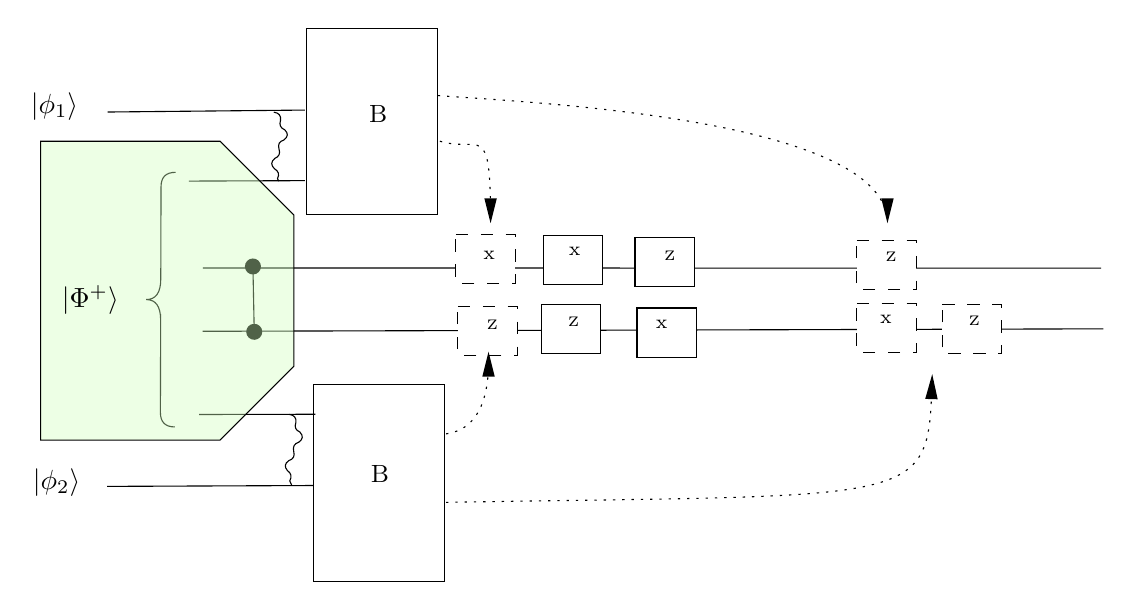
\begin{tikzpicture}[x=0.75pt,y=0.75pt,yscale=-1,xscale=1]
%uncomment if require: \path (0,300); %set diagram left start at 0, and has height of 300

%Shape: Brace [id:dp4160546662329181] 
\draw   (130,95) .. controls (125.33,94.99) and (122.99,97.31) .. (122.98,101.98) -- (122.86,146.31) .. controls (122.84,152.98) and (120.5,156.3) .. (115.83,156.29) .. controls (120.5,156.3) and (122.82,159.64) .. (122.8,166.31)(122.81,163.31) -- (122.68,210.65) .. controls (122.67,215.32) and (124.99,217.66) .. (129.66,217.67) ;
%Straight Lines [id:da8065384733259011] 
\draw    (97.23,65.94) -- (192.33,65) ;
%Shape: Rectangle [id:dp6790608484549128] 
\draw   (192.98,25.57) -- (256.39,25.57) -- (256.39,115.25) -- (192.98,115.25) -- cycle ;
%Straight Lines [id:da34073899408201536] 
\draw    (136.45,99.22) -- (192.33,99) ;
%Straight Lines [id:da3326977952142205] 
\draw    (97.07,246.31) -- (196.33,245.89) ;
%Shape: Rectangle [id:dp4807359036219334] 
\draw   (196.33,292.34) -- (259.74,292.34) -- (259.74,197.33) -- (196.33,197.33) -- cycle ;
%Straight Lines [id:da5430962616562778] 
\draw    (141.33,211.67) -- (197.33,211.56) ;
%Straight Lines [id:da9639318872173184] 
\draw    (143.18,141.07) -- (575.92,141.17) ;
%Straight Lines [id:da22467135117490433] 
\draw    (143.02,171.59) -- (577,170.4) ;
%Shape: Rectangle [id:dp4475966088803329] 
\draw  [fill={rgb, 255:red, 255; green, 255; blue, 255 }  ,fill opacity=1 ] (307.19,125.54) -- (335.82,125.54) -- (335.82,149.17) -- (307.19,149.17) -- cycle ;
%Shape: Rectangle [id:dp01609794668273845] 
\draw  [fill={rgb, 255:red, 255; green, 255; blue, 255 }  ,fill opacity=1 ] (306.21,158.82) -- (334.84,158.82) -- (334.84,182.45) -- (306.21,182.45) -- cycle ;
%Shape: Rectangle [id:dp456238595830335] 
\draw  [fill={rgb, 255:red, 255; green, 255; blue, 255 }  ,fill opacity=1 ] (351.32,126.31) -- (379.95,126.31) -- (379.95,149.94) -- (351.32,149.94) -- cycle ;
%Shape: Rectangle [id:dp6950101334971088] 
\draw  [fill={rgb, 255:red, 255; green, 255; blue, 255 }  ,fill opacity=1 ] (352.3,160.37) -- (380.93,160.37) -- (380.93,184) -- (352.3,184) -- cycle ;
%Shape: Rectangle [id:dp5224143658365781] 
\draw  [fill={rgb, 255:red, 255; green, 255; blue, 255 }  ,fill opacity=1 ][dash pattern={on 4.5pt off 4.5pt}] (265.03,124.76) -- (293.66,124.76) -- (293.66,148.4) -- (265.03,148.4) -- cycle ;
%Shape: Rectangle [id:dp8276974594794448] 
\draw  [fill={rgb, 255:red, 255; green, 255; blue, 255 }  ,fill opacity=1 ][dash pattern={on 4.5pt off 4.5pt}] (458.19,158.05) -- (486.82,158.05) -- (486.82,181.68) -- (458.19,181.68) -- cycle ;
%Shape: Rectangle [id:dp30201259432122174] 
\draw  [fill={rgb, 255:red, 255; green, 255; blue, 255 }  ,fill opacity=1 ][dash pattern={on 4.5pt off 4.5pt}] (499.38,158.82) -- (528.01,158.82) -- (528.01,182.45) -- (499.38,182.45) -- cycle ;
%Shape: Rectangle [id:dp20575966558705927] 
\draw  [fill={rgb, 255:red, 255; green, 255; blue, 255 }  ,fill opacity=1 ][dash pattern={on 4.5pt off 4.5pt}] (458.19,127.86) -- (486.82,127.86) -- (486.82,151.49) -- (458.19,151.49) -- cycle ;
%Shape: Rectangle [id:dp879155044923984] 
\draw  [fill={rgb, 255:red, 255; green, 255; blue, 255 }  ,fill opacity=1 ][dash pattern={on 4.5pt off 4.5pt}] (266.01,159.59) -- (294.64,159.59) -- (294.64,183.23) -- (266.01,183.23) -- cycle ;
%Curve Lines [id:da09246323435174553] 
\draw  [dash pattern={on 0.84pt off 2.51pt}]  (257.33,80) .. controls (277.13,85.94) and (281.67,68.76) .. (281.76,117.99) ;
\draw [shift={(281.76,119.5)}, rotate = 270] [fill={rgb, 255:red, 0; green, 0; blue, 0 }  ][line width=0.08]  [draw opacity=0] (12,-3) -- (0,0) -- (12,3) -- cycle    ;
%Curve Lines [id:da06959625459364571] 
\draw  [dash pattern={on 0.84pt off 2.51pt}]  (256.33,58) .. controls (296,61.12) and (469.45,68.27) .. (472.91,117.98) ;
\draw [shift={(472.97,119.5)}, rotate = 270] [fill={rgb, 255:red, 0; green, 0; blue, 0 }  ][line width=0.08]  [draw opacity=0] (12,-3) -- (0,0) -- (12,3) -- cycle    ;
%Curve Lines [id:da39316974650838654] 
\draw  [dash pattern={on 0.84pt off 2.51pt}]  (260.33,221) .. controls (280.79,218.21) and (280.89,193.07) .. (280.8,183.34) ;
\draw [shift={(280.78,181.42)}, rotate = 90] [fill={rgb, 255:red, 0; green, 0; blue, 0 }  ][line width=0.08]  [draw opacity=0] (12,-3) -- (0,0) -- (12,3) -- cycle    ;
%Curve Lines [id:da18722309143811278] 
\draw  [dash pattern={on 0.84pt off 2.51pt}]  (260.33,254) .. controls (492.98,250.04) and (492.61,256.37) .. (494.48,194.16) ;
\draw [shift={(494.54,192.26)}, rotate = 91.75] [fill={rgb, 255:red, 0; green, 0; blue, 0 }  ][line width=0.08]  [draw opacity=0] (12,-3) -- (0,0) -- (12,3) -- cycle    ;
%Straight Lines [id:da761825964657918] 
\draw    (167.26,140.36) -- (167.89,171.83) ;
\draw [shift={(167.89,171.83)}, rotate = 88.87] [color={rgb, 255:red, 0; green, 0; blue, 0 }  ][fill={rgb, 255:red, 0; green, 0; blue, 0 }  ][line width=0.75]      (0, 0) circle [x radius= 3.35, y radius= 3.35]   ;
\draw [shift={(167.26,140.36)}, rotate = 88.87] [color={rgb, 255:red, 0; green, 0; blue, 0 }  ][fill={rgb, 255:red, 0; green, 0; blue, 0 }  ][line width=0.75]      (0, 0) circle [x radius= 3.35, y radius= 3.35]   ;
%Curve Lines [id:da1435143281948974] 
\draw    (184.75,211.61) .. controls (187.26,211.98) and (188.32,213.33) .. (187.93,215.65) .. controls (187.19,217.76) and (187.83,219.24) .. (189.85,220.09) .. controls (191.59,221.94) and (191.43,223.57) .. (189.37,225) .. controls (187.19,225.67) and (186.37,227.16) .. (186.91,229.47) .. controls (187.52,231.7) and (186.76,233.16) .. (184.63,233.84) .. controls (182.56,235.23) and (182.3,236.84) .. (183.87,238.68) .. controls (185.73,239.95) and (186.11,241.62) .. (185.01,243.69) -- (186.04,245.97) ;
%Curve Lines [id:da2586024030465792] 
\draw    (177.33,66) .. controls (179.84,66.37) and (180.91,67.71) .. (180.54,70.02) .. controls (179.85,72.15) and (180.53,73.65) .. (182.6,74.52) .. controls (184.38,76.25) and (184.23,77.88) .. (182.16,79.43) .. controls (179.98,80.08) and (179.2,81.51) .. (179.82,83.74) .. controls (180.55,85.92) and (179.87,87.44) .. (177.8,88.29) .. controls (175.9,89.89) and (175.84,91.54) .. (177.61,93.24) .. controls (179.62,94.44) and (180.12,96.02) .. (179.1,97.98) -- (179.72,99.27) ;
%Snip Same Side Corner Rect [id:dp59755192438972] 
\draw  [fill={rgb, 255:red, 208; green, 254; blue, 187 }  ,fill opacity=0.39 ] (151.42,80) -- (187,115.58) -- (187,188.42) -- (151.42,224) -- (65,224) -- (65,224) -- (65,80) -- (65,80) -- cycle ;

% Text Node
\draw (317.69,163.54) node [anchor=north west][inner sep=0.75pt]   [align=left] {{\tiny Z}};
% Text Node
\draw (364.12,131.88) node [anchor=north west][inner sep=0.75pt]   [align=left] {{\tiny Z}};
% Text Node
\draw (360.19,165.08) node [anchor=north west][inner sep=0.75pt]  [font=\normalsize] [align=left] {{\scriptsize x}};
% Text Node
\draw (318.2,129.83) node [anchor=north west][inner sep=0.75pt]  [font=\normalsize] [align=left] {{\scriptsize x}};
% Text Node
\draw (277.03,131.76) node [anchor=north west][inner sep=0.75pt]  [font=\normalsize] [align=left] {{\scriptsize x}};
% Text Node
\draw (510.87,163.09) node [anchor=north west][inner sep=0.75pt]   [align=left] {{\tiny Z}};
% Text Node
\draw (470.71,132.36) node [anchor=north west][inner sep=0.75pt]   [align=left] {{\tiny Z}};
% Text Node
\draw (468.12,162.73) node [anchor=north west][inner sep=0.75pt]  [font=\normalsize] [align=left] {{\scriptsize x}};
% Text Node
\draw (278.53,165.09) node [anchor=north west][inner sep=0.75pt]   [align=left] {{\tiny Z}};
% Text Node
\draw (222.01,61.73) node [anchor=north west][inner sep=0.75pt]  [font=\normalsize] [align=left] {{\small B}};
% Text Node
\draw (222.78,234.78) node [anchor=north west][inner sep=0.75pt]  [font=\normalsize] [align=left] {{\small B}};
% Text Node
\draw (59,55.4) node [anchor=north west][inner sep=0.75pt]    {$\ket{\phi _{1}}$};
% Text Node
\draw (60,236.4) node [anchor=north west][inner sep=0.75pt]    {$\ket{\phi _{2}}$};
% Text Node
\draw (74,148.4) node [anchor=north west][inner sep=0.75pt]    {$\ket{\Phi ^{+}}$};


\end{tikzpicture}


 \caption{A CZ-gate circuit that uses quantum teleportation. Using the fact that the CZ gate and the Pauli gates are in the Clifford group, we can commute the CZ gate with the X and Z gates (with some correction) such that this circuit is equivalent to \cref{fig:QTCZ-1}. See \ref{Appendix} for proof. figure adapted from \cite{Kok:2005jip} and \cite{KnillE2001Asfe}. }
    \label{fig:QTCZ-2}
\end{figure}

The important takeaway from this is that we can apply a CZ gate to our inner modes in $\ket{\Phi^+}$, as shown in \cref{fig:QTCZ-2}, \textbf{before} the states $\ket{\phi_1}$ and $\ket{\phi_2}$ are teleported into these modes. This means that if we can prepare a successful $\ket{\Phi^+}$ 'offline', meaning before we put it into our circuit and perform teleportation we run $\ket{\Phi^+}$ multiple times until we have a successful result, then we can apply the teleportation when, and only when we have a successful $\ket{\Phi^+}$. This is significant because in \cref{fig:QTCZ-1} if the CZ gate fails then we have lost the states $\ket{\phi_1}$ and $\ket{\phi_2}$ so the probability of this circuit being correct hinges entirely on the CZ gate \textbf{but} in \cref{fig:QTCZ-2}, if everything highlighted in green is prepared offline, $\ket{\phi_1}$ and $\ket{\phi_2}$ are only teleported after a successful CZ gate operation, we essentially guarantee the success of the entire circuit in \cref{fig:QTCZ-2} and input states aren't destroyed\cite{GottesmanDaniel1999QTia}.
\par
Unfortunately, there's a catch that we've neglected to mention up until now; performing a Bell Measurement is non-deterministic with a probability of $\frac{1}{2}$. Since we perform two Bell Measurements to teleport our two qubit states, the total probability of success for the \cref{fig:QTCZ-2} circuit is $\frac{1}{4}$ which is exactly what we started with. This is where the KLM near-deterministic teleporter comes in. 

\subsubsection{KLM Near Deterministic Teleporter}
Due to the non-deterministic nature of the Bell Basis Measurement, the circuit \cref{fig:QTCZ-2} has a probability of success of $\frac{1}{4}$ but if there is a way we can deterministically (or near deterministically) teleport our input states $\ket{\phi_1}$ and $\ket{\phi_2}$ after a successful CZ gate (prepared offline) is implemented then we have a near deterministic CZ circuit.
\par
For this section alone we'll be considering the single-rail qubit representation as opposed to the dual-rail representation that we've been focused on until now because the CZ gate in single-rail encoding only requires one optical mode and so the picture here should be clearer to see when we teleport one optical mode. The aim is to teleport the initial qubit $\ket{\phi} = \alpha\ket{0} + \beta\ket{1}$.
\par
We start by preparing 2n optical modes and we're going to put them in the superposition state:
    \begin{equation}
        \ket{t_n} = \frac{1}{\sqrt{n+1}}\sum\limits_{j=0}^{n}\ket{1}^j\ket{0}^{n-j}\ket{0}^j\ket{1}^{n-j}
        \label{eqn: QFT Teleporter EQ}
    \end{equation} \cite{KnillE2001Asfe}\cite{Kok:2005jip}
here $\ket{k}^j \equiv \ket{k}_1 \otimes...\otimes\ket{k}_j$ where $\ket{k}_j$ signifies the $j^{th}$ mode being in the state $\ket{k}$ and $\otimes$ represents the tensor product. 
\par
We're going to look at an example where we choose n=5 to see what $\ket{t_n}$ looks like. Remembering that $\ket{t_n}$ represents 2n optical modes, $\ket{t_5}$ describes 10 optical modes.
\begin{equation}
        \ket{t_5} = \frac{1}{\sqrt{5+1}}\sum\limits_{j=0}^5\ket{1}^j\ket{0}^{5-j}\ket{0}^j\ket{1}^{5-j}
    \end{equation}
    \begin{align} 
        \ket{t_5} =  & \ket{0}^{5}\ket{1}^5 
        + \\ & \ket{1}\ket{0}^{4}\ket{0}\ket{1}^{4} + 
 \\ & \ket{1}^2\ket{0}^{3}\ket{0}^2\ket{1}^{3} \label{t5:1} + \\ & \ket{1}^3\ket{0}^{2}\ket{0}^3\ket{1}^{2}\label{t5:2} + \\  & \ket{1}^4\ket{0}\ket{0}^4\ket{1} + \\ & \ket{1}^{5}\ket{0}^5  
 \label{eqn: t5 breakdown}
\end{align}
\textit{note: we've neglected the preceding normalisation term for conciseness but each of the states in the $\ket{t_n}$ superposition have equal probability }
\par
If we look at just one of the lines above, \cref{eqn: t5 breakdown}, for example, $\ket{1}^5\ket{0}^5$ and explicitly write it as a string of 0's and 1's representing whether a photon is present in a given optical mode then if $\ket{t_5} = \ket{1}^5\ket{0}^5$:
    \begin{equation}
        \ket{t_5} = 1111100000
    \end{equation}
In this example the first 5 optical modes \footnote{and therefore the first 5 qubits since this is single-rail encoding} in $\ket{t_5}$ have a photon present whilst the latter 5 have none.
\par 
As you can see, $\ket{t_5}$ is a superposition of all of these states when we prepare it. In our near deterministic teleporter, we put the first n modes (in our example, the first 5) as well as the input mode $\ket{\phi}$ (the state we want to teleport) into the discrete Quantum Fourier Transform (QFT).  We haven't discussed the discrete QFT in detail and it goes beyond the scope of this report but there are two important results to know from applying it:
\begin{itemize}
    \item after inputting n+1 modes the QFT will output 1 singular mode with "m" photons
    \item these m photons come from our input modes but the information about which exact modes they came from is destroyed, the 'which-path' information is erased.
\end{itemize}
So after the input mode $\ket{phi}$ and the first n modes of $\ket{t_n}$ are put through the QFT, the output 'm' tells us there are m photons in these first n+1 modes, we then find that the $(n+m)^{th}$ mode has the exact state of $\ket{\phi}$. This is shown diagrammatically in \cref{fig:Near deterministic tele}. To see this clearly we go back to our example of $\ket{t_5}$.
\par
Imagine, after applying the QFT over $\ket{\phi} (= \alpha\ket{0} + \beta\ket{1}$) and $\ket{t_5}$, the output is m=3. Logically we know then that either 1 photon came from $\ket{\phi}$ (in which case the other 2 came from the first 5 modes of $\ket{t_5}$) or 0 photons came from $\ket{\phi}$ (in which case all 3 came from the first 5 modes of $\ket{t_5}$). Due to the QFT destroying 'which-path' information, we don't know which of these two cases our output corresponds to but we know it can only be one of these two. This means that the only contributions to $\ket{t_5}$ from our large sum are \cref{t5:1} and \cref{t5:2}. With the modes for each circuit written explicitly, these two possibilities are:
 \begin{alignat*}{0}
        &\mathbf{0} \quad  &  &\mathbf{1 2 3 4 5}  \quad &  &\mathbf{6 7 8 9 (10)}\\
        \alpha \;\;\;  &0 \quad &  &0 1 1 1 0 0  \quad  &  &1 1 {\color{red}0} 0 0 \\
        \beta  \;\;\; &1 \quad  &  &1 1 1 0 0 0 \quad &  &1 1 {\color{red}1} 0 0 \\
\end{alignat*}
where the bold numbers are labels for each mode and $\alpha$ and $\beta$ are the amplitudes for each possibility. The zeroth column represents our input qubit $\ket{\phi}$, columns 1-5 represent the first 5 modes of $\ket{t_5}$ and columns 6-10 represent the last 5 modes of $\ket{t_5}$.
\par
The 'teleportation' happens when we look at the $(n+m)^{th}$ mode, in our case this is the 8th column as highlighted in red above.  We can see that this column is exactly the same as the zeroth column (our input mode). We have just teleported our input mode into the 8th mode of our circuit. 
\par
As you might have guessed, our QFT is not deterministic, it fails when the output m is equal to 0 or n+1 because in these cases we know the input state $\ket{\phi}$ collapsed and there is only one possible outcome of the $\ket{t_5}$ superposition our circuit could be in but since these are only 2 cases if we increase the number of modes n, the chances of m= 0,(n+1) diminishes. More explicitly we can say that as we increase the number of modes in the circuit in \cref{fig:Near deterministic tele} the probability, $= \frac{n}{n+1}$, approaches one.

\begin{figure}[H]
    \centering
    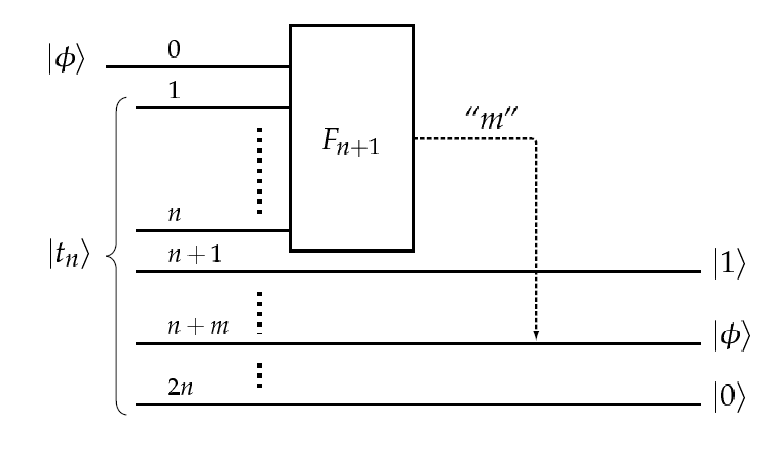
\includegraphics[scale=0.5]{images/Near Deterministic Teleporter.png}
    \caption{Circuit for the Near Deterministic Teleporter proposed by KLM. The Quantum Fourier transform takes the input and n modes of the prepared state $\ket{t_n}$ to produce an output mode with m photons. The $(n+m)^{th}$ mode of the circuit is where we will find our teleported input state. figure taken from \cite{Kok:2005jip}}
    \label{fig:Near deterministic tele}
\end{figure}

\subsubsection{Bringing it all together}
%Now we have seen how the KLM protocol makes quantum teleportation a near-deterministic process, 
In this section, the viability of photonic quantum computers is discussed. Going back to the DiVincenzo Criteria, for this approach to even be considered, it is crucial that is satisfies all five criteria. First of all, in an optical quantum computer the qubit is represented by the location of a photon in one of two spacial modes. It is possible to initialise the system by creating photons in a well defined state. This is can be done by attenuating laser light. Furthermore, the output of the quantum computer can be easily read out with the use of photo detectors. As per the fourth requirement, a set of universal quantum gates is achieved by combining linear optical elements, such as beamsplitters and phase shifters, with either nonlinear Kerr media or by implementing the probabilistic KLM protocol. Finally, photons have long decoherence times, which makes it difficult for them to lose their quantum properties. However, this same property is also the reason why it is complicated to make them interact and why a protocol as complex as KLM is needed in order to implement two qubit gates. Thus, all five of the DiVincenzo criteria can be met. 

In Linear Optical Quantum Computing we encode our qubits using the spacial positions of photons the state being determined by whether they are in one tube (rail/ mode) or another. We can then perform single qubit quantum logic gates to these qubits by using classical linear optical tools that act on photons, these include beamsplitters, phase shifters, mirrors, etc. To create a Universal Set of quantum logic gates we need to implement 2 qubit quantum logic gates which are gates that act on 2 qubits. These are difficult to do in photonic quantum computing because photons hardly interact with each other but using the Hong-Ou-Mandel effect we can create logic gates that are probabilistic; they sometimes 'fail' and give us a random output. These probabilistic logic gates make photonic quantum computing look like a method that can't scale due to the fact that with large circuits with many gates, the chances of these gates not failing is exponentially slim. Gottesman and Chuang introduced a trick to overcome this by suggesting that if we use Quantum Teleportation, we can prepare probabilistic gates (such as the control z gate) ahead of time and 'teleport' the states we want to apply these gates to when necessary. This trick is essential at making photonic quantum computing seem viable but it is hindered by the fact that Bell Measurements (which are a vital step in Quantum Teleportation) are also probabilistic. This is where Knill, Leflamme and Milburn introduce the near-deterministic teleporter which can perform the teleportation in the Gottesmann and Chuang trick to near 100\% accuracy so long as a large number of resources are used, these resources will always be less exhaustive  than the alternative (creating new photons to send into our circuit until we finally get a successful result). In this way we can create a Quantum Computer which uses qubits that rarely lose their states (due to the minimal interactions photons have with the general environment), can be operated at room temperature, has qubits that can be easily operated on (using linear optical tools) and that can be scaled (using the KLM protocol). Considering all these factors, it would be feasible to conclude that LOQC is a highly viable approach for quantum computing.

\begin{center}
    \Huge \textbf{Old notes and scrap space}
\end{center}
\vspace{-1em}

\section{Jans notes}
Ok, I'm taking over this section for now
\begin{itemize}

\item
Found this thing called DiVincezo criteria which might be nice to mention or something, it's 5 criteria that need to be met for a given hypothetical quantuum computer implementation:
\begin{itemize}
    \item A physical system containing well-defined 2 level quantum systems (qubits) which can be isolated from the environment.
    \item The ability to initialize this system in a well defined, determinate state.
    \item A set of universtal quantum gates which can be applied to each qubit or possibly pairs (or more) of them.
    \item Qubit decoherence times much greater than times for quantum gates to be applied.
    \item The ability to read out qubit state with high accuracy.
    \item ** In addition 2 more were mentioned by him, the ability to convert between "stationary" (like trapped ions) and "flying" (photons) states which would be necessary for a quantum network.
\end{itemize}

\item
    The Nielsen book lists quite a few of physical implementations for quantum computers - QHO, optical photon, optical cavity, ion traps and nuclear magnetic resonance

\item Trapped ion systems, kinda taken from Bruzewicz 2019, they also mention the DiVincezo stuff
\begin{itemize}
    \item All the main parts have been demonstrated, the problem is scaling.
    \item The actual states are the electronic states of some atom/ion.
    \item A couple types: hyperfine, Zeeman, fine structure and optical the differences between them is the particular energy levels that are used for states.
            The names make it decently clear, fine structure means the fine structure split states are used, optical means states which are transitioned between by photon emission/absorption.
    \item One of the things to deal with is that the atoms energies come from both their structure and their motion within the trap (which is also quantized).
    \item Some of the manipulations take place through lasers.
    \item Main pros are long coherence time and great gate and initialization/readout fidelity, drawbacks include speed, the gates are quite slow compared to other qubit technologies.
    \item Unordered random facts
    \begin{itemize}
        \item single qubit gates take a couple micro seconds and double about 10-100 micro seconds
        \item coherence times range from 0.2 to 600s (600s achieved for hyperfine) and surface code error correction was mentioned, the gate fielity should be good enough for that
        \item with respect to the optional DiVincezo, ions are unlikely to be the "flying" ones even though they can be moved, however high-fielity entanglement between ions and photons has been showed.
        \item most of the main things have been demonstrated by 2004 though the maximum number of ions achieved in a register so far was 20.
    \end{itemize}

    \item As far as I understand it is in fact a single ion that would represent a given qubit, the obvious way to store them are Penning or Paul traps.
    \item Paul traps rely on time dependent quadrupole fields (oscillating, usually trig or square waveforms).
    \item Penning traps do a mix of E and B fields to get a fairly complicated but alright motion.
    \item As far as I can tell Paul traps are considered the easier ones (and are more developed) but Penning traps have their advantages.

    \item Paul traps
    \begin{itemize}
        \item There are in fact 2 types.
        \item Point Paul traps have oscillating traps in all 3 dimensions, resulting in a single point with net 0 RF force (over a period).
            This can lead to issues when trapping multiple ions in the same trap as they tend to interact/overlap a lot.
        \item Linear Paul traps are the other type, they have an RF quadrupole in 2 dimensions and a static electric potential across the last one, this means the atoms can space better along that line according to that static potential.
        \item Okay, it's actually kinda insanely cool, so nowadays instead of it actually being 4 rods for the quadrupole field and some segments for the static field, they can deform this onto a surface -- as in the trap itself is a little plate with conducting segments to which the voltages are applied.
            Apparently it's still a good enough field and it is easy to make, there is plenty access for lasers and so on.
    \end{itemize}
    \item Atoms are loaded using resonant photo-ionization to make sure only a given isotope is present (in the past bombarding the atom gas with electrons as used and resulted in different isotopes being in the trap)
    \item Typically the excite states are quite high energy and multiple steps might be needed (often using near UV photons) to get them there.
    \item Apparently mostly elements from the 2nd group in the periodic table (or ones with similar properties) are used for trapped ion qubits.
    \item Any 2 states with long lifetimes can be used for the 0 and 1 states and almost always one of them is from the "ground state manifold" and based on where the other is the energy splittings can be anything between MHz to hundreds of THz.
    \begin{itemize}
        \item A big aspect of linear paul trap based systems is how it results in essentially a 1D crystal with the ions all trapped in the same harmonic potential along the axis, this results in shared motional states
        \item As we've just done in ICMP, there can be vibrational modes aka phonons which are "shared" among the ions (sorry don't have a simple but more formal explanation for now).
        \item There are 3N vibrational modes for this sort of a crystal with N ions and each mode is in a harmonic oscillator state (as in can be in a superposition of different harmonic oscillator states).
        \item The article I'm readidng now mentions that "lasers can be used to excite the internal electronic levels dependent upon the ions' vibrational states" which I'm not sure how but I see how that would lead to a way to entangle their states.
    \end{itemize}

    \item So I now skipped to more of the overview/applicability part.
    \item We might want to mention NISQ (Noisy Itentermeiate-Scale Quantum computing) -- it is a term describing the type of quantum computer we might be able to build now or in the very near future.
        It is essentially a subfield, studying what useful applications they could have is done. They require about 100s of qubits and as far as I can tell they "do not handle error correction" by themselves, the algorithms need to take care of that.
    \item A 53 qubit trapped ion system was used for further physics research (as far as I can understand they used it to simulate some complicate quantum many body system, they call is a quantum simulator).
    \item Quantum simulations using quantum computers seems to be a big thing in general, the Nature Physics 2012 Insight collections intro mentions atomic quantum gases, trapped ions, photonic systems and superconducting circuits being demonstrated.
    \item And I have seen a couple mentions of ~10s (up to 20 or so) qubit trapped ion systems though I didn't track them down right now.
\end{itemize}

\section{Trapped Ion Quantum Computing}
In this section we provide an introduction to the implementation details of trapped ion quantum computers (**once done possibly elaborate what exactly we covered).
The qubits in a trapped ion system are represented by individual trapped ions, as would have been seen in a quantum mechanics class, electrons bound in atoms can occupy a certain number of possible quantum states, here 2 of these level are chosen and used as the \kz and \ko states.
Though it isn't quite as simple as that, for quantum computing we must have a way of entangling these 2 states.
To achieve that, the qubits are trapped in the same trap (this will be explained further later on) and their motion within it is coupled as a quantum system through which entanglement is achieved.
Finally for qubit manipulation, lasers are used to excite and cool down the electrons and the ions themselves.

\subsection{Ion Trapping and the Paul Trap}
Ion trapping is an extensive field of expertise used for many purposes across physics and other sciences, it is an essential component of many experiments that try to manipulate individual particles, molecules or so on.
For a brief sketch of what this involves, these experiments must be done in vacuum (otherwise there would be too many other atoms around) and rely on complex electric and magnetic fields to manipulate the motion of charged atoms.
For quantum computing we are interested in trapping individual ions in a stable way, and while we want to trap multiple of them (currently about 5-100 has been achieved !43) it is important that we can tell them apart (as opposed to trapping them in bunches as is often done).

There are currently 2 dominant suitable ion trap designs, the Penning trap which uses a combination of magnetic and electric fields, and the Paul trap which uses time varying electric fields.
Penning traps are able to hold larger amounts of ions and more stably (300 ion crystals have been achieved !46), however the motion of the ions themselves is much more complicated and leads to qubit manipulation being harder to perform.
Because of that Paul traps are more commonly used for quantum computers and due to the scope of this report we will mainly focus on them.

\subsubsection{Simple Paul Trap}
Paul trap designs use time varying fields as it is not possible to confine an ion in 3D space with only static fields.
The simplest Paul trap design is composed of 4 conducting rods run in parallel to create a quadrupole electric field in the middle.
Then have each of the diagonally opposite rods connected at the same voltage and have these 2 voltages be some periodic function (usually a sine or a square wave) in antiphase, so that if at some time one is set to positive voltage, the other should be at negative voltage (**hopefully add a diagram/picture).
This results in a net effect of trapping a charged particle (within some range of mass to charge ratios, this setup is also called the Radio-Frequency-Quadrupole and can be used as a mass filter) along the axis of the quadrupole, why exactly this is well explained in (**add a source here).
Finally, for trapping along the last axis a static electric field is used, this can be achieved by for example 2 more rod segments along the quadrupole axis at either end of the whole setup, both at some positive voltage, resulting in a 


\subsubsection{Notes on Advanced Paul Trap designs}


% There are many different ways of constructing a Paul trap, different electrode geometries give different benefits and downsides.

% For quantum computing we are mainly interested to trap individual ions in a predictable and stable way, there are 2 main types of ions traps that are used, the Penning tr



\end{itemize}

\section{Michael's Section}
Finding a physical representation of qubits that fulfil all the mathematical requirements is not easy.
Gaining control over a single quantum system has been a want since about 1970. word this so better
It is possible to see quantum effects on a vast number of combined quantum systems such as in superconductors. \cite{nielsen_quantum_2010}
Or in particle collisions again quantum effects are observed however there isn't control over a single quantum system.
Qubits are the physical realisation of controlling a single quantum system and its state.
You require a system with many degrees of freedom that can encode quantum information (qubits). \cite{bergou_quantum_2021}

\subsection{Optical Photon Quibit}

Why Photons?
\begin{itemize}
    \item Photons are massless, chargeless and don't interact with each other or other mass much. \cite{nielsen_quantum_2010}
    \item Can be guided long distances without much energy loss using optical fibers. \cite{nielsen_quantum_2010}
    \item Quantum information can be transmitted over long distances using photons as demonstrated by quantum entanglement over 1200km. \cite{yin_satellite-based_2017}
    \item photons can maintain entanglement over long distances and time period allowing the transmission quantum information. - this supper secure wow \cite{thibault_team_nodate}
\end{itemize}


How photons?

\begin{itemize}
    \item The transverse polarisation state of a photon can be used to represent qubits. 
    These are vertical, horizontal linear and left, right circular polarization. \cite{bergou_quantum_2021}
    \item These states can also be maintained - in isotropic materials photons polarization does not change as it propagates. \cite{bergou_quantum_2021}
    \item $\left\langle 0 \right\vert $
\end{itemize}


\printbibliography

\end{document}
